%% Copernicus Publications Manuscript Preparation Template for LaTeX Submissions
%DIF LATEXDIFF DIFFERENCE FILE
%DIF DEL viejo.tex   Mon Jan 14 22:03:23 2019
%DIF ADD nuevo.tex   Mon Jan 14 22:02:51 2019
%% ---------------------------------
%% This template should be used for copernicus.cls
%DIF 4c4
%DIF < %% The class file and some style files are bundled in the Copernicus Latex Package which can be downloaded from the different journal webpages.
%DIF -------
%% The class fil e and some style files are bundled in the Copernicus Latex Package which can be downloaded from the different journal webpages. %DIF > 
%DIF -------
%% For further assistance please contact the Copernicus Publications at: publications@copernicus.                                                                                         x    
%% http://publications.copernicus.org


%% Please use the following documentclass and Journal Abbreviations for Discussion Papers and Final Revised Papers.


%% 2-Column Papers and Discussion Papers
%++++++++++++++++++++++35\documentclass[nhess, manuscript]{copernicus}
%\documentclass[nhess]{copernicus}
%DIF 15c15
%DIF < \documentclass[hessd, manuscript]{copernicus}
%DIF -------
\documentclass[hess, manuscript]{copernicus} %DIF > 
%DIF -------


%% Journal Abbreviations  (Please use the same for Discussion Papers and Final Revised Papers)

% Atmospheric Chemistry and Physics (acp)
% Advances in Geosciences (adgeo)
% Advances in Statistical Climatology, Meteorology and Oceanography (ascmo)
% Annales Geophysicae (angeo)
% ASTRA Proceedings (ap)
% Atmospheric Measurement Techniques (amt)
% Advances in Radio Science (ars)
% Advances in Science and Research (asr)
% Biogeosciences (bg)
% Climate of the Past (cp)
% Drinking Water Engineering and Science (dwes)
% Earth System Dynamics (esd)
% Earth Surface Dynamics (esurf)
% Earth System Science Data (essd)
% Fossil Record (fr)
% Geographica Helvetica (gh)
% Geoscientific Instrumentation, Methods and Data Systems (gi)
% Geoscientific Model Development (gmd)
% Geothermal Energy Science (gtes)
% Hydrology and Earth System Sciences (hess)
% History of Geo- and Space Sciences (hgss)
% Journal of Sensors and Sensor Systems (jsss)
% Mechanical Sciences (ms)
% Natural Hazards and Earth System Sciences (nhess)
% Nonlinear Processes in Geophysics (npg)
% Ocean Science (os)
% Primate Biology (pb)
% Scientific Drilling (sd)
% SOIL (soil)
% Solid Earth (se)
% The Cryosphere (tc)
% Web Ecology (we)



%% \usepackage commands included in the copernicus.cls:
%\usepackage[german, english]{babel}
%\usepackage{tabularx}
%\usepackage{cancel}
%\usepackage{multirow}
%\usepackage{supertabular}
%\usepackage{algorithmic}
%\usepackage{algorithm}
%\usepackage{float}
%\usepackage{subfig}
%\usepackage{rotating}
\usepackage{color}
\definecolor{mypink}{RGB}{219, 48, 122}
%DIF PREAMBLE EXTENSION ADDED BY LATEXDIFF
%DIF UNDERLINE PREAMBLE %DIF PREAMBLE
\RequirePackage[normalem]{ulem} %DIF PREAMBLE
\RequirePackage{color}\definecolor{RED}{rgb}{1,0,0}\definecolor{BLUE}{rgb}{0,0,1} %DIF PREAMBLE
\providecommand{\DIFadd}[1]{{\protect\color{blue}\uwave{#1}}} %DIF PREAMBLE
\providecommand{\DIFdel}[1]{{\protect\color{red}\sout{#1}}}                      %DIF PREAMBLE
%DIF SAFE PREAMBLE %DIF PREAMBLE
\providecommand{\DIFaddbegin}{} %DIF PREAMBLE
\providecommand{\DIFaddend}{} %DIF PREAMBLE
\providecommand{\DIFdelbegin}{} %DIF PREAMBLE
\providecommand{\DIFdelend}{} %DIF PREAMBLE
%DIF FLOATSAFE PREAMBLE %DIF PREAMBLE
\providecommand{\DIFaddFL}[1]{\DIFadd{#1}} %DIF PREAMBLE
\providecommand{\DIFdelFL}[1]{\DIFdel{#1}} %DIF PREAMBLE
\providecommand{\DIFaddbeginFL}{} %DIF PREAMBLE
\providecommand{\DIFaddendFL}{} %DIF PREAMBLE
\providecommand{\DIFdelbeginFL}{} %DIF PREAMBLE
\providecommand{\DIFdelendFL}{} %DIF PREAMBLE
%DIF END PREAMBLE EXTENSION ADDED BY LATEXDIFF

\begin{document}

\linenumbers

\title{Reconstructing the Salgar 2015 Flash Flood Using Radar Retrievals and a Conceptual Modeling Framework: A Basis for a Better Flood Generating Mechanisms Discrimination}


% \Author[affil]{given_name}{surname}

\Author[1,2]{Nicolás Velásquez}{}
\Author[1,2]{Carlos D. Hoyos}{}
\Author[1]{Jaime I. Vélez}{}
\Author[2]{Esneider Zapata}{}

\affil[1]{Universidad Nacional de Colombia, Sede Medellín, Facultad de Minas, Departamento de Geociencias y Medio Ambiente}
\affil[2]{Sistema de Alerta Temprana de Medellín y el Valle de Aburrá (SIATA)}


%% The [] brackets identify the author with the corresponding affiliation. 1, 2, 3, etc. should be inserted.

\runningtitle{Reconstructing the 2015 Flash Flood event of Salgar}

\runningauthor{N. Velásquez}
\correspondence{Nicolás Velásquez (nvelasqg@unal.edu.co)}



\received{}
\pubdiscuss{} %% only important for two-stage journals
\revised{}
\accepted{}
\published{}

%% These dates will be inserted by Copernicus Publications during the typesetting process.


\firstpage{1}

\maketitle


\begin{abstract}
\DIFdelbegin \DIFdel{Flash floods associated with severe precipitation events are highly destructive, often resulting in significant human and economic losses. Due to their nature, flash floods tend to occur in medium to small basins located within complex high mountainous regions. In the Colombian Andean region these basins are common, with the aggravating factor that the vulnerability is considerably high due to the presence of important human settlements frequently occupying floodplains and other flash-flood prone areas.  }\DIFdelend During May 18 of 2015, severe rainfall \DIFdelbegin \DIFdel{generated }\DIFdelend \DIFaddbegin \DIFadd{triggered }\DIFaddend a flash flood in the municipality of Salgar,  \DIFdelbegin \DIFdel{in La Liboriana basin }\DIFdelend located in the northwestern Colombian Andes\DIFdelbegin \DIFdel{, resulting in more than 100 human casualties and significant economic losses}\DIFdelend . This work aims to reconstruct the \DIFdelbegin \DIFdel{2015 La Liboriana }\DIFdelend \DIFaddbegin \DIFadd{main features of the }\DIFaddend flash flood to understand better the hydrological processes \DIFdelbegin \DIFdel{that took place during the event and to serve as a proof of concept for the development of a flash flood guidance low-cost tool when information is scarce. Radar QPE}\DIFdelend \DIFaddbegin \DIFadd{modulating the event occurrence. Radar quantitative precipitation estimates (QPE)}\DIFaddend , satellite data, and post-event field visits are used to reconstruct the Salgar flash flood addressing the relationship between rainfall spatio-temporal structure, soil moisture, and runoff generation during successive rainfall events, using \DIFaddbegin \DIFadd{a }\DIFaddend conceptual modeling framework including land-slide and hydraulic sub-models. The \DIFdelbegin \DIFdel{hydrological model includes the addition of }\DIFdelend \DIFaddbegin \DIFadd{hydrologic model includes }\DIFaddend virtual tracers to explore the role of runoff and subsurface flow, as well as the relative importance of convective and stratiform precipitation in flash flood generation. \DIFdelbegin \DIFdel{The }\DIFdelend \DIFaddbegin \DIFadd{In spite of potential shortcomings, the modeling results allow an }\DIFaddend assessment of the \DIFaddbegin \DIFadd{impact of the }\DIFaddend interactions between runoff, subsurface flow, and convective-stratiform rainfall \DIFdelbegin \DIFdel{allows a better understanding of }\DIFdelend \DIFaddbegin \DIFadd{on }\DIFaddend the short-term hydrological mechanisms leading to the flash flood event.  The overall methodology reproduces considerably well the magnitude and timing of La Liboriana flash flood discharge peak, as well as the areas of \DIFdelbegin \DIFdel{regional land-slide }\DIFdelend \DIFaddbegin \DIFadd{landslide }\DIFaddend occurrence and flood spots\DIFdelbegin \DIFdel{location}\DIFdelend , with some limitations due to the \DIFdelbegin \DIFdel{available spatial scale of the }\DIFdelend digital elevation model \DIFaddbegin \DIFadd{spatial resolution}\DIFaddend . Simulation results indicate that the flash-flood and the regional land-slide features were strongly influenced by the antecedent rainfall associated with a northeasterly stratiform event that recharged the gravitational and capillary storages \DIFdelbegin \DIFdel{. The hydrologic }\DIFdelend \DIFaddbegin \DIFadd{within the model. The }\DIFaddend simulation shows that the antecedent \DIFdelbegin \DIFdel{event set wet conditions in }\DIFdelend \DIFaddbegin \DIFadd{rainfall event moistens }\DIFaddend the entire basin before the occurrence of the flash flood event, \DIFdelbegin \DIFdel{governing }\DIFdelend \DIFaddbegin \DIFadd{modulating as well }\DIFaddend the streamflow during the flash flood event. Evidence suggests that the spatial structure of the rainfall is at least as important as the geomorphological features of the basin \DIFdelbegin \DIFdel{regulating the generation }\DIFdelend \DIFaddbegin \DIFadd{in regulating the occurrence }\DIFaddend of flash flood events. 
\DIFdelbegin \DIFdel{Results also suggest that the described model-based tool is useful for policy-makers not only for short-term decisions in the context of an early warning system but also as a planning resource for long-term risk management. }%DIFDELCMD < \\\\
%DIFDELCMD < 

%DIFDELCMD < %%%
\DIFdelend \end{abstract}
%%-----------------------------------------------------------
%%-----------------------------------------------------------
%Introduction
%%-----------------------------------------------------------
%%-----------------------------------------------------------


\introduction  %% \introduction[modified heading if necessary]

Flash floods are regarded as one of the most destructive hydrological hazards resulting in considerable loss of human life and high costs due to infrastructure \DIFdelbegin \DIFdel{damages  \mbox{%DIFAUXCMD
\citep{Roux2011, Gruntfest2001}}\hspace{0pt}%DIFAUXCMD
.  }\DIFdelend \DIFaddbegin \DIFadd{damage  \mbox{%DIFAUXCMD
\citep{Roux2011, Gruntfest2001}}\hspace{0pt}%DIFAUXCMD
.  Among all different types of floods,  \mbox{%DIFAUXCMD
\cite{Jonkman2005} }\hspace{0pt}%DIFAUXCMD
shows that flash floods result in the highest average mortality rate per event (3.62\%), almost ten times larger than the mortality rate for river floods.  }\DIFaddend Flash floods are usually described as rapidly rising water level events happening in \DIFaddbegin \DIFadd{steep }\DIFaddend streams and rivers, associated with short-term, very intense convective precipitation systems, or orographically forced rainfall events over highly saturated land surfaces and steep terrains \citep{Salek2006, Llasat2016, Douinot2016}.  Convective precipitation episodes often feature high \DIFdelbegin \DIFdel{intensities, short durations}\DIFdelend \DIFaddbegin \DIFadd{intensity, short duration}\DIFaddend , and relatively reduced spatial coverage \citep{HouzeMCS2004}.   \DIFdelbegin \DIFdel{\mbox{%DIFAUXCMD
\cite{Jonkman2005}}\hspace{0pt}%DIFAUXCMD
, based on information from the International Disaster Database, maintained by the United States Office for Foreign Disaster Assistance and the Center for Research on the Epidemiology of Disasters in Brussels, shows that between 1975 and 2001 a total of 1816 worldwide freshwater flood events killed over 175, 000 persons and affected more than 2.2 billion people. These events not only caused human and economic losses but also damages to ecosystems and loss of historical and cultural values. Among all different types of floods,  \mbox{%DIFAUXCMD
\cite{Jonkman2005} }\hspace{0pt}%DIFAUXCMD
shows that flash floods result in the highest average mortality rate per event (3.62\%), almost ten times larger than the mortality rate for river floods.  }\DIFdelend \\

\DIFdelbegin \DIFdel{Several studies assess the role of rainfall, geomorphological features and soil conditions on flash floods occurrence from different points of view. \mbox{%DIFAUXCMD
\citet{Wu1995} }\hspace{0pt}%DIFAUXCMD
highlight }\DIFdelend \DIFaddbegin \DIFadd{Several authors have assessed the role of the geological and geomorphological features of the catchment, soil type,  soil moisture conditions, and the spatio-temporal structure of rainfall on flash flood occurrence, trying to identify the leading causative mechanisms of this hazard \mbox{%DIFAUXCMD
\citep{Merz2003}}\hspace{0pt}%DIFAUXCMD
.  \mbox{%DIFAUXCMD
\citet{Adamovic2016} }\hspace{0pt}%DIFAUXCMD
and \mbox{%DIFAUXCMD
\citet{Vannier2016}  }\hspace{0pt}%DIFAUXCMD
tried to understand the governing processes of flash floods from the geological formation of the basin with mixed results. \mbox{%DIFAUXCMD
\citet{Wu1995} }\hspace{0pt}%DIFAUXCMD
emphasize }\DIFaddend the role of the topography, ground cover, and groundwater in the occurrence of shallow landslides and associated debris flows. \DIFdelbegin \DIFdel{\mbox{%DIFAUXCMD
\citet{Merz2003} }\hspace{0pt}%DIFAUXCMD
highlighted the importance of understanding the physical processes giving rise to floods of a certain probability of occurrence and proposed a framework, from a catchment perspective, for identifying causative mechanisms of inundations and the viability for a large number of episodes and basins}\DIFdelend \DIFaddbegin \DIFadd{Due to their rapid nature, flash floods are more likely to occur in small and steep basins \mbox{%DIFAUXCMD
\citep{Younis2008}}\hspace{0pt}%DIFAUXCMD
; many authors have assessed the influence of hills and stream slopes suggesting the slopes of the hills are significantly more important for flash floods occurrence and magnitude than the slope of the stream  \mbox{%DIFAUXCMD
\citep{Salek2006, Roux2011, Yatheendradas2008}}\hspace{0pt}%DIFAUXCMD
. \mbox{%DIFAUXCMD
\citet{Rodriguez2012}  }\hspace{0pt}%DIFAUXCMD
analyzed fifty-four flash flood episodes in Spain and determined that antecedent soil moisture conditions play a vital role in runoff production.  \mbox{%DIFAUXCMD
\citet{Castillo2003}}\hspace{0pt}%DIFAUXCMD
, using a modeling approach, also suggested an important flash flood occurrence dependence on antecedent moisture conditions. \mbox{%DIFAUXCMD
\citet{Aronica2012} }\hspace{0pt}%DIFAUXCMD
used spatial and statistical analysis to reconstruct landslides and deposits, finding a connection between flash flood occurrence and soil moisture antecedent conditions.}\\

\DIFadd{The fact that small basins are more prone to flash floods increases their intrinsic physical and measurement uncertainty \mbox{%DIFAUXCMD
\citep{Wagener2007}}\hspace{0pt}%DIFAUXCMD
,  difficulting their prediction \mbox{%DIFAUXCMD
\citep{Hardy2016, Ruiz-Villanueva2013, Yamanaka2017,Borga2011, Marra2017}}\hspace{0pt}%DIFAUXCMD
, and underlining the need for high spatio-temporal resolution precipitation data \mbox{%DIFAUXCMD
\citep{Norbiato2008}}\hspace{0pt}%DIFAUXCMD
}\DIFaddend .  Given the critical role of precipitation, some authors follow a climatological approximation to assess the recurrence of flash floods in particular regions\DIFdelbegin \DIFdel{and study the different }\DIFdelend \DIFaddbegin \DIFadd{, focusing on the }\DIFaddend atmospheric causative mechanisms. \DIFdelbegin \DIFdel{These studies have evidenced the need to incorporate global and regional climatological conditions and variability in local risk reduction. }\DIFdelend For example, \citet{Kahana2002} examined the extent to which floods in the Negev Desert are the outcome of \DIFdelbegin \DIFdel{distinct }\DIFdelend climatological synoptic-scale features finding that about 80\% of the events can be linked to distinct synoptic \DIFdelbegin \DIFdel{types characterized by the prevailing atmospheric }\DIFdelend conditions days prior the flood events.  \citet{Schumacher2005} studied extreme rain events associated with flash flooding in the United States over a 3-yr period using the national radar reflectivity composite data \DIFdelbegin \DIFdel{are }\DIFdelend to examine the structure and evolution of each extreme rain events. \DIFaddbegin \DIFadd{The use of radar data to study flash flood generating storms is vital for understanding and forecasting these events  (National Research Council 1996).  }\DIFaddend \citet{Schumacher2005}  found that 65\% of the total number of episodes are associated with mesoscale convective systems (MCSs), with two recurrent patterns of organization: the existence of training convective elements and the generation of quasi-stationary areas of convection with stratiform rainfall downstream.  \citet{Fragoso2012} analyzed storm characteristics and required rainfall conditions for flash flood occurrence at Madeira (Portugal), and their results suggest an essential role of global climate patterns (North Atlantic Oscillation -NAO- forcing) and also local forcing (orographic features) in the triggering of such events.  \DIFdelbegin \DIFdel{\mbox{%DIFAUXCMD
\citet{Piper2016} }\hspace{0pt}%DIFAUXCMD
examined the critical elements of flash flood triggering storms following a statistical approach, finding an essential role of stationary convective cores. \mbox{%DIFAUXCMD
\citet{Gochis2015} }\hspace{0pt}%DIFAUXCMD
studied the great Colorado flood of 2013, documenting not only the meteorological conditions but also the climatological ones responsible for producing the observed widespread destruction, associating them with the potential for sustaining a  blocking ridge over the Canadian Rockies and a slow-moving, cutoff, upper-level cyclonic circulation to its south over the western United States. Implicitly, all the studies mentioned }\DIFdelend \DIFaddbegin \DIFadd{Implicitly, these studies }\DIFaddend and all the others available in the peer-reviewed literature point to the need for local and regional \DIFdelbegin \DIFdel{quality }\DIFdelend \DIFaddbegin \DIFadd{high-quality  }\DIFaddend spatio-temporal rainfall data. \citet{BERNE2013} highlight the need to incorporate high-resolution weather radar information, even with some limitations, in flash flood hydrology. \\

\DIFdelbegin \DIFdel{Different authors have shown that antecedent soil moisture significantly influences the occurrence and behavior of flash floods.   \mbox{%DIFAUXCMD
\citet{Rodriguez2012}  }\hspace{0pt}%DIFAUXCMD
analyzed fifty-four flash flood episodes in Spain and determined that antecedent conditions are a vital point in runoff production.  \mbox{%DIFAUXCMD
\citet{Castillo2003}}\hspace{0pt}%DIFAUXCMD
, using a modeling approach, highlighted the role of antecedent moisture conditions in flash flood occurrence associating them with different kinds of storm events. \mbox{%DIFAUXCMD
\citet{Aronica2012} }\hspace{0pt}%DIFAUXCMD
used spatial and statistical analysis to reconstruct landslides and deposits, finding a connection between flash flood occurrence and soil moisture antecedent conditions. \mbox{%DIFAUXCMD
\citet{Tramblay2012b} }\hspace{0pt}%DIFAUXCMD
showed better flash flood model performance when using remotely sensed soil moisture data as initial conditions in a hydrological modeling study. Other authors have tried to understand the governing processes of flash floods from the geological formation of the basin \mbox{%DIFAUXCMD
\citep{Adamovic2016, Vannier2016}}\hspace{0pt}%DIFAUXCMD
.}%DIFDELCMD < \\
%DIFDELCMD < 

%DIFDELCMD < %%%
\DIFdel{Due to the rapid nature of flash floods, they are more likely to occur in small and steep basins \mbox{%DIFAUXCMD
\citep{Younis2008}}\hspace{0pt}%DIFAUXCMD
, highlighting the need for the availability of detailed temporal scale precipitation data \mbox{%DIFAUXCMD
\citep{Norbiato2008} }\hspace{0pt}%DIFAUXCMD
and high-resolution terrain information. Watersheds prone to these events are usually located in rural mountainous areas with poor gauge information (rain and level). The utilization of radar data to study flash flood generating storms is vital for understanding and forecasting these events  (National Research Council 1996).  One of the most critical challenges associated with flash floods is their simulation and prediction \mbox{%DIFAUXCMD
\citep{Yamanaka2017,Borga2011, Marra2017}}\hspace{0pt}%DIFAUXCMD
. The fact that flash floods are more prone in small basins increases their intrinsic physical and measurement uncertainty \mbox{%DIFAUXCMD
\citep{Wagener2007}}\hspace{0pt}%DIFAUXCMD
,  difficulting their prediction \mbox{%DIFAUXCMD
\citep{Hardy2016,Ruiz-Villanueva2013}}\hspace{0pt}%DIFAUXCMD
.  Many authors have assessed the influence of hills and stream slopes and evidence suggest the slopes of the hills are significantly more important for flash floods occurrence and magnitude than the stream slope \mbox{%DIFAUXCMD
\citep{Doswell2001, Salek2006, Roux2011, Yatheendradas2008}}\hspace{0pt}%DIFAUXCMD
.}%DIFDELCMD < \\
%DIFDELCMD < 

%DIFDELCMD < %%%
\DIFdel{Arguably one of the most meaningful applications of quantitative precipitation estimation (QPE)  from a societal point of view is its use to improve flash flood forecasting. The use of weather radar QPE products in flash flood applications could potentially offset, in part, the lack of in-situ precipitation products in small poorly gauged basins and become an important stepping stone for improving the state-of-the-art understanding of flash flood processes such as orographically enhanced extreme rainfall events and runoff generation \mbox{%DIFAUXCMD
\citep{Creutin2003}}\hspace{0pt}%DIFAUXCMD
.  However, in some cases, there still exist limitations associated with the spatial resolution of radar retrievals \mbox{%DIFAUXCMD
\citep{Salek2006, Hardy2016}}\hspace{0pt}%DIFAUXCMD
. Nevertheless, several modern approaches involving radar information, in-situ precipitation data, model approximations and merging algorithms are promising \mbox{%DIFAUXCMD
\citep{Braud2016}}\hspace{0pt}%DIFAUXCMD
.}%DIFDELCMD < \\
%DIFDELCMD < 

%DIFDELCMD < %%%
\DIFdelend The topography of Colombia is characterized by three branches of the Andes crossing the country south-to-north, generating a mixture of landscapes from high snow-capped mountains, vast highland plateaus, deep canyons to wide valleys,  making some regions highly prone to flash flood occurrence. The likelihood of flash flood occurrence in Colombia is also high due to the spatio-temporal behavior of the Intertropical Convergence Zone, and the direction of the near-surface moist air flow leading to orographic enhancement of convective cores  \citep{Poveda2007}. In the last decade, there have been several widespread and localized flash flood events in Colombia associated with climatological features and with the local intensification of rainfall events.  The 2010-2011 La Niña event alone triggered 1233 flooding events and 778 mass removal processes \DIFaddbegin \DIFadd{in Colombia}\DIFaddend ,  with more than 3 million people affected and damages estimated  by the "Comisión Económica para América Latina y el Caribe" in more than 6.5 billion US dollars.\DIFdelbegin \DIFdel{After this }\DIFdelend \DIFaddbegin \\

\DIFadd{After the  2010-2011 }\DIFaddend widespread disaster, several \DIFdelbegin \DIFdel{localized }\DIFdelend \DIFaddbegin \DIFadd{isolated }\DIFaddend events have occurred in the country with devastating consequences. \DIFdelbegin %DIFDELCMD < \\
%DIFDELCMD < 

%DIFDELCMD < %%%
\DIFdel{Between May 15th and May 18th, 2015, several storms took place over La Liboriana basin located in the municipality of Salgar, in the department of Antioquia (Colombia). By 2015, the population of Salgar was estimated at 17400 persons, 8800 residing in the urban area.  La Liboriana is a small tropical basin(}\DIFdelend \DIFaddbegin \DIFadd{The present paper focuses on studying the processes triggering a flash flood in La Liboriana basin,  a }\DIFaddend 56 \DIFdelbegin \DIFdel{$km^2$) }\DIFdelend \DIFaddbegin \DIFadd{km$^2$  basin }\DIFaddend located in the western range \DIFdelbegin \DIFdel{(Cordillera Occidental) }\DIFdelend of the Colombian Andes\DIFdelbegin \DIFdel{. During the night of May 17th, between 02:00 and 09:00 A.M. (local time), a precipitation event covered almost all the basin (hereafter referred to as event 1).  Twenty hours later, between 23:00 P.M of }\DIFdelend \DIFaddbegin \DIFadd{, as a result of consecutive rainfall storms that took place between May 15th and }\DIFaddend May \DIFdelbegin \DIFdel{17 and 02:00 A.M. of May 18 two successive extreme convective systems occurred over the basin with the maximum intensity in the upper hills (event 2).  Event 1 corresponds mainly to a stratiform event, covering almost all the basin area and with an average precipitation accumulation of 47 $mm$. Event 2 accumulated, averaging over the basin, around 38 $mm$, however over the upper watershed the accumulation exceeded 180 $mm$. The occurrence of these successive rainfall events resulted in a flash flood that took }\DIFdelend \DIFaddbegin \DIFadd{18th, 2015. The resulting flash flood dramatically affected the region, causing }\DIFaddend more than 100 \DIFdelbegin \DIFdel{human lives and affected }\DIFdelend \DIFaddbegin \DIFadd{casualties,   affecting }\DIFaddend several buildings and critical infrastructure\DIFdelbegin \DIFdel{.  The total investment for the reconstruction of Salgar´s infrastructure and the psychosocial attention of the community is }\DIFdelend \DIFaddbegin \DIFadd{, and resulting in a total reconstruction cost }\DIFaddend estimated at 36.000 million Colombian pesos (approximately 12,5 million dollars considering 2018 exchange rate), which corresponds to three times the annual income of the municipality.  Figure \ref{fig:Antes_y_Despues} shows an example of infrastructure damage as a result of the flash flood event, and \DIFdelbegin \DIFdel{satellite images }\DIFdelend \DIFaddbegin \DIFadd{changes }\DIFaddend of the basin's main channel \DIFdelbegin \DIFdel{before and }\DIFdelend after the flash flood, showing considerable river \DIFdelbegin \DIFdel{margins }\DIFdelend \DIFaddbegin \DIFadd{margin }\DIFaddend and bed erosion. \DIFaddbegin \DIFadd{In spite of the data scarcity, including discharge measurements, the analysis of the successive rainfall events triggering the Salgar flash flood  provide an interesting case of study for assessing the mechanisms depending on the soil moisture conditions and rainfall distribution.}\DIFaddend \\


\begin{figure}[t]
    \centering
    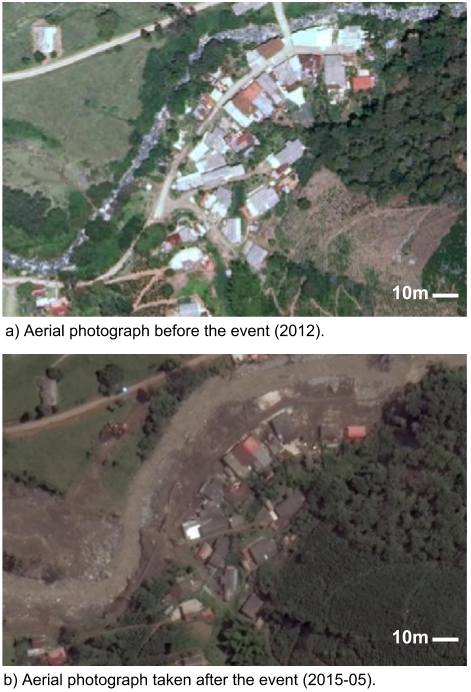
\includegraphics[width=8.3cm]{Figures/Salgar_Before_After.png}
    \caption{Example of infrastructure damage as a result of the La Liboriana May 18 of 2015 flash flood event. a) Aerial photograph before the event (2012) taken during a mission of the Department of Antioquia´s Government, and b) satellite image after the event (2015-05). The images show the destruction of most houses in that particular community, a bridge over La Liboriana, and the main road. The images also present changes in the delineation of the main channel as well as considerable erosion in the river margins.}
    \label{fig:Antes_y_Despues}
\end{figure}

La Liboriana basin flash flood is a typical case of prediction in ungauged basins  \DIFdelbegin \DIFdel{(PUB) }\DIFdelend \citep{Sivapalan2013, Seibert2009, Beven2007, Bonell2006, Yamanaka2017}.  In this case,  there are no local records of soils or land use and the local hydro-meteorological data is scarce or non-existent and certainly not available in real time. Due to the lack of data, La Liboriana case imposes a challenge for flash flood prediction and modeling. According to \citet{blschl2012}, there are three methods for using models in \DIFdelbegin \DIFdel{PUB }\DIFdelend \DIFaddbegin \DIFadd{these }\DIFaddend cases. The first strategy is to obtain the required model parameters from historical basin behavior and the morphological characteristics of the basin. This strategy often leads to low model performance \citep{Duan2006}. The second approach is to inherit the hydrological calibration from a gauged neighboring watershed, which in this case does not exist. The third method is to parameterize the model based on proxy variables, such as hydraulic information obtained during field \DIFdelbegin \DIFdel{recognition}\DIFdelend \DIFaddbegin \DIFadd{visits}\DIFaddend . In the case of the 2015 La Liboriana basin flash flood, there are no previous historical streamflow records, nor records from a neighboring watershed\DIFdelbegin \DIFdel{.}%DIFDELCMD < \\
%DIFDELCMD < 

%DIFDELCMD < %%%
\DIFdel{The present work aims to reconstruct the 2015 La Liboriana flash flood, not only to understand better the hydrological processes that took place during the event but also to serve as a proof of concept that hopefully leads to the development of a flash flood guidance low-cost tool based on the scarce information existent. Such a tool should be useful for decision-makers not only for short-term decisions in the context of an early warning system but also as a planning resource for long-term risk management. In particular, this workuses }\DIFdelend \DIFaddbegin \DIFadd{, thus we followed the third approach. In this work, we use precipitation }\DIFaddend information derived from radar\DIFdelbegin \DIFdel{QPE, satellite data}\DIFdelend \DIFaddbegin \DIFadd{, satellite and aereal images}\DIFaddend , and post-event field visits to reconstruct the Salgar flash flood event. \DIFdelbegin \DIFdel{Also, this }\DIFdelend \DIFaddbegin \DIFadd{This }\DIFaddend study addresses two broad hydrological issues. The first issue consists in exploring the relationship between rainfall spatio-temporal structure \citep{Llasat2016,Fragoso2012}, soil moisture and runoff generation \citep{Penna2011,Tramblay2012b,Garambois2013} during the successive rainfall events\DIFdelbegin \DIFdel{. The second issue consists }\DIFdelend \DIFaddbegin \DIFadd{, and the second issue }\DIFaddend in proposing a simplified \DIFdelbegin \DIFdel{hydrological }\DIFdelend \DIFaddbegin \DIFadd{hydrologic }\DIFaddend modeling scheme including land-slide and hydraulic sub-models to \DIFdelbegin \DIFdel{detect and anticipate potential }\DIFdelend \DIFaddbegin \DIFadd{assess the potential occurrence of }\DIFaddend flash flood events.\\

The methodology followed in this study makes use of a conceptual modeling framework that includes a \DIFdelbegin \DIFdel{hydrological model }\DIFdelend \DIFaddbegin \DIFadd{hydrologic model \mbox{%DIFAUXCMD
\citep{Velez2001, Frances2007b}}\hspace{0pt}%DIFAUXCMD
}\DIFaddend , a shallow land-slide sub-model \DIFaddbegin \DIFadd{\mbox{%DIFAUXCMD
\citep{Aristizabal2016}}\hspace{0pt}%DIFAUXCMD
}\DIFaddend , and a hydraulic sub-model \DIFdelbegin \DIFdel{. The hydrological model,  based on the work by \mbox{%DIFAUXCMD
\citet{Velez2001} }\hspace{0pt}%DIFAUXCMD
and \mbox{%DIFAUXCMD
\citet{Frances2007b}}\hspace{0pt}%DIFAUXCMD
,  simulates different hydrological processes as independent but interacting storages. The shallow landslide sub-model follows the formulation described in \mbox{%DIFAUXCMD
\citep{Aristizabal2016}}\hspace{0pt}%DIFAUXCMD
. The hydraulic sub-model corresponds to a low-cost 1D model }\DIFdelend (hereafter referred to as HydroFlash)\DIFdelbegin \DIFdel{that assumes infinite sediment supply and estimates the cross-sectional filled area at all time steps. The hydrological model includes the addition of }\DIFdelend \DIFaddbegin \DIFadd{. The hydrologic model includes }\DIFaddend virtual tracers to explore separately the role of runoff and subsurface flow, as well as the relative importance of convective and stratiform precipitation in flash flood generation. The \DIFdelbegin \DIFdel{convective and stratiform classification follows the methodology proposed by \mbox{%DIFAUXCMD
\citet{Houze2015} }\hspace{0pt}%DIFAUXCMD
and \mbox{%DIFAUXCMD
\citet{Steiner1995}}\hspace{0pt}%DIFAUXCMD
. The }\DIFdelend assessment of the interactions between runoff, subsurface flow, and convective-stratiform rainfall allows a better understanding of the short-term hydrological mechanisms leading to the flash flood event.  \DIFdelbegin \DIFdel{The model is parameterized using field information from a river cross-section located at the entrance of the urban area of Salgar. }\DIFdelend A comparison between the results from both sub-models and the observed landslides scars and flooded spots helps to evaluate the overall skill of the proposed methodology. \\

The document is structured as follows. Section \ref{sec:data} describes in more detail the region of study, La Liboriana basin, including geomorphological and climatological characteristics of the basin as well as the information sources used in this study. Section \ref{sec:methods} presents a description of the overall methodology and the model used for the reconstruction of the 2015 La Liboriana flash flood event, including flow separation, shallow landslide parameterization, and the proposed hydraulic model. Section \ref{sec:results} describes the main results of the study, including model \DIFdelbegin \DIFdel{parameterization and validation . Section \ref{sec:results} also }\DIFdelend \DIFaddbegin \DIFadd{validation and sensitivity analysis, and presents results from the land-slide and inundation sub-models. Section \ref{sec:discussion} }\DIFaddend includes a discussion on the role of the rainfall structure in the flash flood reconstruction\DIFdelbegin \DIFdel{and presents results from the land-slide and inundation sub-models}\DIFdelend .  Finally,  the conclusions are presented in section \ref{sec:conclusions}.

\section{\DIFdelbegin \DIFdel{Data and Area of }\DIFdelend Study \DIFaddbegin \DIFadd{Site and Data}\DIFaddend }
\label{sec:data}

\DIFaddbegin \subsection{\DIFadd{Catchment description}}

\DIFaddend The urban area of Salgar municipality is located near the outlet of La Liboriana basin, a small (56 \DIFdelbegin \DIFdel{$km^2$}\DIFdelend \DIFaddbegin \DIFadd{km$^2$}\DIFaddend ) tropical watershed located in the westernmost range of Colombia's Andes (Figure \ref{fig:Ubicacion}).  \DIFaddbegin \DIFadd{By 2015, the population of Salgar was estimated at 17400 persons, 8800 residing in the urban area.  }\DIFaddend La Liboriana basin joins El Barroso river basin and both drain to Cauca river. \DIFaddbegin \\

\DIFaddend The availability of the ALOS-PALSAR Digital Elevation Model (DEM) \citep{ALOS}, with a resolution of about 12.7 \DIFdelbegin \DIFdel{$m$}\DIFdelend \DIFaddbegin \DIFadd{m}\DIFaddend , allows estimating the fundamental geomorphological features \DIFaddbegin \DIFadd{of the basin}\DIFaddend . The average slope of La Liboriana is  57.6 \%, and the basin longitude and perimeter are 13.5 \DIFdelbegin \DIFdel{$km$ }\DIFdelend \DIFaddbegin \DIFadd{$\text{km}$ }\DIFaddend and 57.8 \DIFdelbegin \DIFdel{$km$}\DIFdelend \DIFaddbegin \DIFadd{$\text{km}$}\DIFaddend , respectively.  The Strahler-Horton order of the \DIFdelbegin \DIFdel{principal }\DIFdelend \DIFaddbegin \DIFadd{main }\DIFaddend stream is 5, and \DIFdelbegin \DIFdel{the }\DIFdelend \DIFaddbegin \DIFadd{its }\DIFaddend longitude and slope \DIFdelbegin \DIFdel{of the principal stream }\DIFdelend are 18.1 \DIFdelbegin \DIFdel{$km$ }\DIFdelend \DIFaddbegin \DIFadd{$\text{km}$ }\DIFaddend and 8.1 \%\DIFaddbegin \DIFadd{, }\DIFaddend respectively. The highest elevation of the watershed (Cerro Plateado) reaches 3609 meters above sea level (m.a.s.l), while the outlet of the basin is at 1316 m.a.s.l..  The \DIFdelbegin \DIFdel{longitudinal profile (see Figure \ref{fig:Perfil}) exhibits considerable steepness in the upper basin. The }\DIFdelend 99th slope percentile of order 1 streams is 78\%. For streams order 2, 3, 4, and 5\DIFaddbegin \DIFadd{, }\DIFaddend the 99th slope percentile are 61, 27, 18 y 11\%, respectively. \DIFaddbegin \DIFadd{Figure \ref{fig:Ubicacion} shows the spatial distribution of the slopes in the watershed. }\DIFaddend These features are typical of Andean mountainous basins.  \DIFdelbegin \DIFdel{The hypsometric curve shows considerable elevation changes for a cumulative area below 33\% (see blue line in Figure \ref{fig:Perfil}). }\DIFdelend Geomorphologically, this kind of watershed \DIFdelbegin \DIFdel{is }\DIFdelend \DIFaddbegin \DIFadd{tends to be }\DIFaddend prone to the occurrence of flash floods \DIFaddbegin \DIFadd{\mbox{%DIFAUXCMD
\citep{Lehmann2012, Penna2011, Martin2018,Longoni2016, Ozturk2018, Khosravi2018, Marchi2016, Bisht2018}}\hspace{0pt}%DIFAUXCMD
}\DIFaddend .\\

\DIFdelbegin %DIFDELCMD < \begin{figure}[t]
%DIFDELCMD < \centering
%DIFDELCMD <     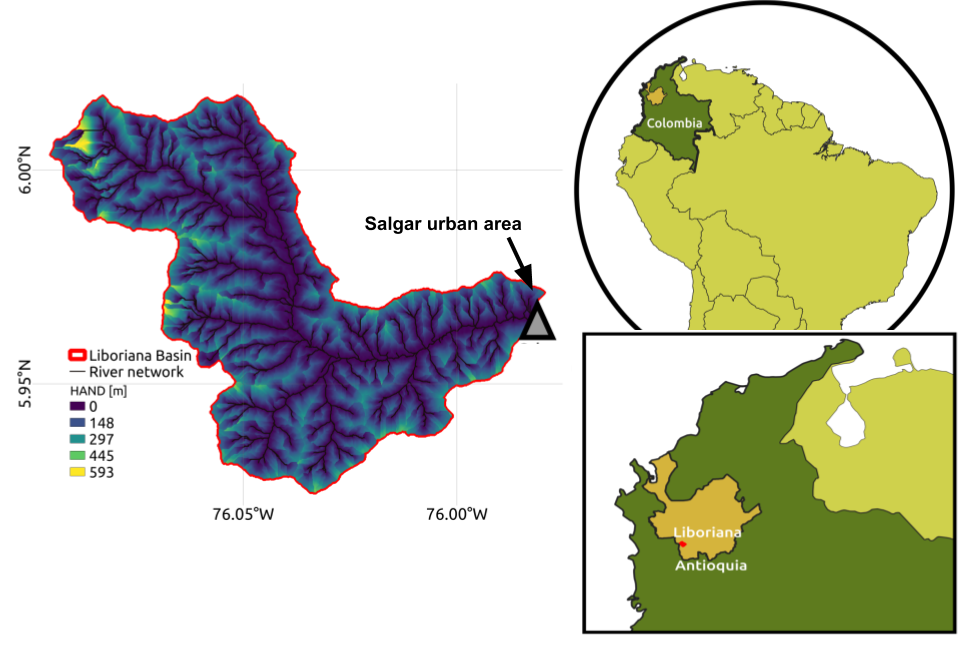
\includegraphics[width=8.3cm]{Figures/Ubicacion.png}
%DIFDELCMD <     %%%
%DIFDELCMD < \caption{%
{%DIFAUXCMD
\DIFdelFL{Geographical context of Liboriana basin,  located in Colombia, in the Department of Antioquia.  The color bar represents the Height Above the Nearest Drainage (HAND).  Low HAND values correspond to areas prone to flooding.}}
    %DIFAUXCMD
%DIFDELCMD < \label{fig:Ubicacion}
%DIFDELCMD < \end{figure}
%DIFDELCMD < %%%
\DIFdelend %DIF > The longitudinal profile (see Figure \ref{fig:Perfil}) exhibits considerable steepness in the upper basin.
%DIF > The hypsometric curve shows considerable elevation changes for a cumulative area below 33\%   (see blue line in Figure \ref{fig:Perfil}).  

At the sub-basin scale, La Liboriana exhibits a vast range of slopes and altitude differences.  Figure \ref{fig:Ubicacion} shows the Height Above the Nearest Drainage -HAND- model   \citep{Renno2008} for La Liboriana. The HAND calculates the relative difference between cell $i$ and its nearest streamflow cell $j$.  La Liboriana HAND exhibits values between 500 and 800 \DIFdelbegin \DIFdel{$m$}\DIFdelend \DIFaddbegin \DIFadd{$\text{m}$}\DIFaddend . Near the outlet of the basin, over the banks, there are values close to 0 m.  High HAND values at the upper region of the watershed often denote areas of high potential energy, with increased sediment production and frequent shallow \DIFdelbegin \DIFdel{landslides }\DIFdelend \DIFaddbegin \DIFadd{landslide }\DIFaddend occurrence.  Banks with low HAND values are more susceptible to flooding and tend to correspond to areas prone to extensive damages caused by extreme events.  While the elevation differences described in Figure \ref{fig:Ubicacion} are typical of the region, the social challenges lie in the high vulnerability of \DIFdelbegin \DIFdel{the }\DIFdelend Salgar given the location of the main urban settlement.\\ 

\begin{figure}[t]
\centering
    \DIFdelbeginFL %DIFDELCMD < 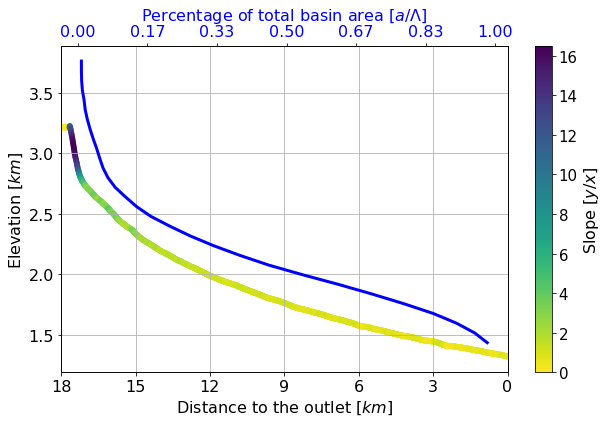
\includegraphics[width=8.3cm]{Figures/Perfil_Cauce.png}
%DIFDELCMD <     %%%
\DIFdelendFL \DIFaddbeginFL 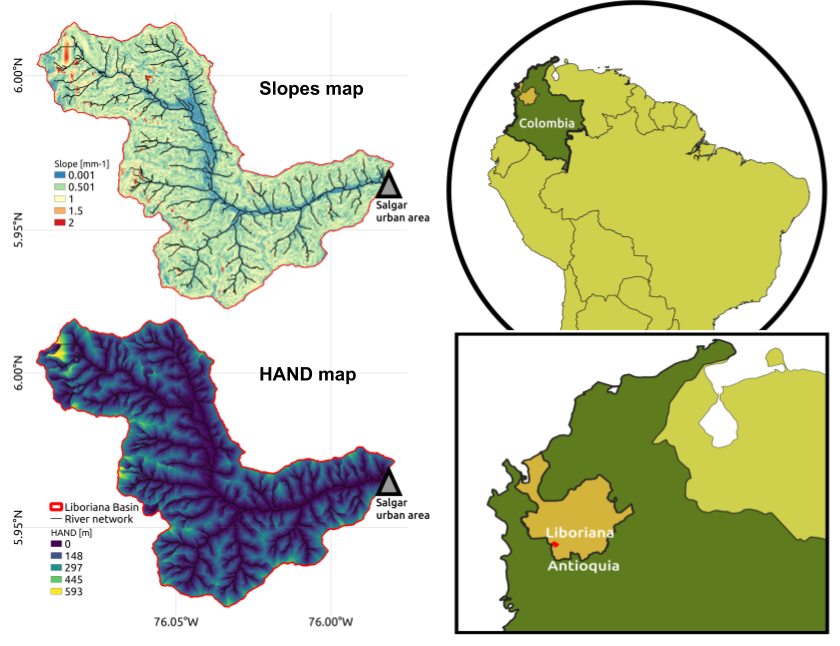
\includegraphics[width=12cm]{Figures/UbicacionV2.png}
    \DIFaddendFL \caption{\DIFdelbeginFL \DIFdelFL{Longitudinal profile }\DIFdelendFL \DIFaddbeginFL \DIFaddFL{Geographical context }\DIFaddendFL of \DIFaddbeginFL \DIFaddFL{Liboriana basin,  located in Colombia, in }\DIFaddendFL the \DIFdelbeginFL \DIFdelFL{principal stream (colored line) from the upper part }\DIFdelendFL \DIFaddbeginFL \DIFaddFL{Department }\DIFaddendFL of \DIFaddbeginFL \DIFaddFL{Antioquia.  The color bar represents }\DIFaddendFL the \DIFdelbeginFL \DIFdelFL{basin to its outlet at }\DIFdelendFL \DIFaddbeginFL \DIFaddFL{Height Above }\DIFaddendFL the \DIFdelbeginFL \DIFdelFL{entrance of }\DIFdelendFL \DIFaddbeginFL \DIFaddFL{Nearest Drainage (HAND).  HAND values where estimated using }\DIFaddendFL the \DIFdelbeginFL \DIFdelFL{urban area, hypsometric curve }\DIFdelendFL \DIFaddbeginFL \DIFaddFL{same resolution }\DIFaddendFL of the \DIFdelbeginFL \DIFdelFL{drainage basin }\DIFdelendFL \DIFaddbeginFL \DIFaddFL{DEM }\DIFaddendFL (\DIFdelbeginFL \DIFdelFL{blue line}\DIFdelendFL \DIFaddbeginFL \DIFaddFL{12.7 $\text{m}$}\DIFaddendFL ).  \DIFaddbeginFL \DIFaddFL{Low HAND values correspond to areas prone to flooding.}\DIFaddendFL }
    \DIFdelbeginFL %DIFDELCMD < \label{fig:Perfil}
%DIFDELCMD < %%%
\DIFdelendFL \DIFaddbeginFL \label{fig:Ubicacion}
\DIFaddendFL \end{figure}


%DIF > \begin{figure}[t]
%DIF > \centering
 %DIF >    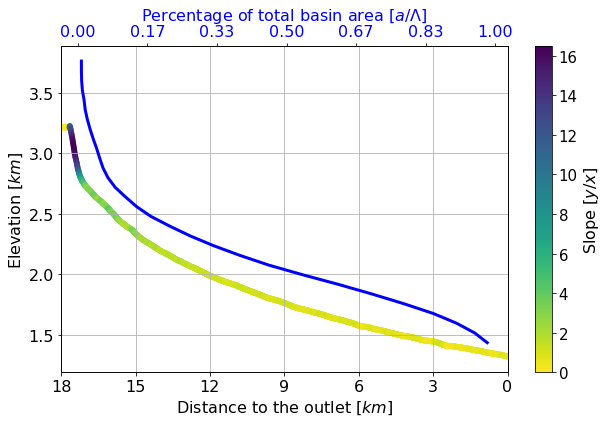
\includegraphics[width=8.3cm]{Figures/Perfil_Cauce.png}
 %DIF >    \caption{Longitudinal profile of the principal stream (colored line) from the upper part of the basin to its outlet at the entrance of the urban area, hypsometric curve of the drainage basin (blue line).}
 %DIF >    \label{fig:Perfil}
%DIF > \end{figure}
\DIFaddbegin 

\DIFaddend Vegetation and land use vary considerably within the basin. \DIFaddbegin \DIFadd{Figure \ref{fig:landuse} shows land use in different regions of the watershed from a 2012 aereal image. }\DIFaddend In the upper La Liboriana basin, there \DIFdelbegin \DIFdel{are crop fields and tropical forests; a }\DIFdelend \DIFaddbegin \DIFadd{is dense vegetation (see Zoom 1 in Figure \ref{fig:landuse}), with a high percentage of tropical forests, with the presence of grass and few crop fields.  A }\DIFaddend portion of the \DIFaddbegin \DIFadd{upper }\DIFaddend watershed is considered a national park. Hillslopes near the divide do not evidence significant anthropic intervention most likely due steepness of \DIFdelbegin \DIFdel{the slopes in }\DIFdelend this region.  Down the hills and at the bottom of the valley there are coffee plantations (the primary economic activity of the region) and pastures.  \DIFaddbegin \DIFadd{Downstream (Figure \ref{fig:landuse}, Zoom 2), it is evident the presence of crops among forest and grass. Near the middle of the basin (Figure \ref{fig:landuse}, Zoom 3), the presence of crops is more notorious and human settlements and roads start to appear. }\DIFaddend The watershed exhibits grazing areas and urban development near the river banks.  \DIFaddbegin \DIFadd{In Figure \ref{fig:landuse}, Zoom 4, corresponding to the first affected urban area from upstream to downstream during the flash flood, it is also possible to see a marked presence of crops and some forest patches.  Finally, zoom 5 shows the main urban area of Salgar surrounded by crops, grass and an important loss of forest coverage. }\DIFaddend \\

\DIFdelbegin \DIFdel{The Andean Colombian region tends to present well-developed soils of different textures with a predominance of limes and clays.  }\DIFdelend \DIFaddbegin \begin{figure}[t]
\centering
\includegraphics[width=12cm]{Salgar_VegetationDetails.png}
\caption{\DIFaddFL{Land use in different regions of La Liboriana watershed from a 2012 aereal images (Source: Department of Antioquia.}}
\label{fig:landuse}
\end{figure}


\DIFaddend One of the challenges for hydrological modeling and risk management in the country is that soils are not well mapped; \DIFaddbegin \DIFadd{the }\DIFaddend national soil cartography is usually available in \DIFaddbegin \DIFadd{a }\DIFaddend 1:400.000 scale. At this scale, the municipality of Salgar, including La Liboriana basin,  corresponds to only one \DIFaddbegin \DIFadd{category of }\DIFaddend soil texture. \DIFdelbegin \DIFdel{The only available information corresponds to descriptions by regional authorities. \mbox{%DIFAUXCMD
\citet{Osorio2008}}\hspace{0pt}%DIFAUXCMD
describe }\DIFdelend \DIFaddbegin \DIFadd{\mbox{%DIFAUXCMD
\citet{Osorio2008}}\hspace{0pt}%DIFAUXCMD
, based on field campaign observations and laboratory tests, described }\DIFaddend La Liboriana soils as \DIFaddbegin \DIFadd{a }\DIFaddend well-drained \DIFaddbegin \DIFadd{soil }\DIFaddend with poor retention capacity.  Organic material is predominant in the first layer and clay loam soil within the second one.  The depth of the soil is hillslope dependent, varying \DIFdelbegin \DIFdel{between }\DIFdelend \DIFaddbegin \DIFadd{from }\DIFaddend 20$cm$ \DIFdelbegin \DIFdel{and }\DIFdelend \DIFaddbegin \DIFadd{to }\DIFaddend 1$m$ \citep{Osorio2008}. Table \ref{tab:suelos} provides a summary of soil characteristics for five different categories, all as a function of slope. Each soil category has a corresponding depth and a qualitative description of permeability and retention.\\

\begin{table}[t]
  \caption{Description of the soils in the region \citep{Osorio2008}.}
  \begin{tabular}{lcccr}
  \hline
    \textbf{Type} & \textbf{Slope} & \textbf{Depth [$m$]} & \textbf{Retention} & \textbf{Permeability} \\    
  \hline
    \textbf{Class III} & 12-25 & 0.6 & Mean & Mean \\
    \textbf{Class IV} & <12 & 0.6 & Low & High \\
    \textbf{Class VI} & 25-30 & 1.0 & Mean & Mean \\
    \textbf{Class VII} & 30-50 & 0.3 & Too Low & Slow \\
    \textbf{Class VIII} & >50 & 0.2 & Too Low & Slow \\
  \hline
  \end{tabular}
%   \belowtable{The description given by the IGAC institute is subjective, without mentioning exact values of retention and permeability.  The depth values given are approximations.} % Table Footnotes
  \label{tab:suelos}
\end{table}

\DIFdelbegin \DIFdel{A field campaign }\DIFdelend \DIFaddbegin \subsection{\DIFadd{Flash flood post-event observations}}

\DIFadd{We conducted a field campaign a }\DIFaddend few days after the \DIFaddbegin \DIFadd{May 18th }\DIFaddend flash flood event \DIFdelbegin \DIFdel{was instrumental in obtaining }\DIFdelend \DIFaddbegin \DIFadd{to assess }\DIFaddend cross-section geometry along the main channel \DIFaddbegin \DIFadd{in different sites}\DIFaddend , including at the outlet of the basin. \DIFdelbegin \DIFdel{The }\DIFdelend \DIFaddbegin \DIFadd{Unfortunately, most of the affected areas were not accessible after the event and it was not  possible to obtain reliable information in other locations along the main channel other than at the outlet of the basin. During the campaign, we measured sectional distances and surface water speeds at different points of the streamflow. We also identified traditional post-event terrain, land-cover, vegetation and infrastructure markers to assess the high-water marks associated with the peak of the flash flood.  Figure \ref{fig:Seccion} presents the selected }\DIFaddend cross-section \DIFaddbegin \DIFadd{used for the estimation of the maximum discharge during the flash flood given its geometrical and hydraulic regularity. The section }\DIFaddend has a rectangular shape,  \DIFdelbegin \DIFdel{and it is }\DIFdelend 4.6 \DIFdelbegin \DIFdel{$m$ wide and has }\DIFdelend \DIFaddbegin \DIFadd{$\text{m}$ wide and }\DIFaddend a height of 5 \DIFdelbegin \DIFdel{$m$ }\DIFdelend \DIFaddbegin \DIFadd{$\text{m}$ }\DIFaddend for a total area of about 23 \DIFdelbegin \DIFdel{$m^2$}\DIFdelend \DIFaddbegin \DIFadd{$\text{m}^2$}\DIFaddend . A visual inspection of the flooded \DIFdelbegin \DIFdel{infrastructure around this section}\DIFdelend \DIFaddbegin \DIFadd{house around the section,   located 4-5 $\text{m}$ away from the channel, }\DIFaddend reveals the presence of mud marks on the walls with heights varying between 0.5 and 1.2 \DIFdelbegin \DIFdel{$m$. These mud stains are evident in buildings located 4-5 $m$ away from the channel }\DIFdelend \DIFaddbegin \DIFadd{$\text{m}$ }\DIFaddend (see Figure \ref{fig:Seccion}). The area of the section plus the flooded area during the event was estimated to be approximately 37 \DIFdelbegin \DIFdel{$m^2$.  Assuming flow speeds }\DIFdelend \DIFaddbegin \DIFadd{$\text{m}^2$.  During the campaign we measured surface speeds in the channel oscillating between 2 and 3 $\text{ms}^{-1}$.   In instrumented basins in the region, with similar characteristics in terms of area and slopes,  we have recorded peak flow surface water speeds oscillating }\DIFaddend between 5 and \DIFdelbegin \DIFdel{6 $m/s$, the total discharge required to generate }\DIFdelend \DIFaddbegin \DIFadd{7 $\text{ms}^{-1}$.  By assuming an area of 37 $\text{m}^2$ and the mentioned surface speeds,  we estimate that }\DIFaddend the observed flash flood \DIFdelbegin \DIFdel{vary }\DIFdelend \DIFaddbegin \DIFadd{peak flow may have been }\DIFaddend between 185 and 222 \DIFdelbegin \DIFdel{$m^3/s$. In this work, the soil information and the field campaign are used to parametrize a hydrological model}\DIFdelend \DIFaddbegin \DIFadd{$\text{m}^3\text{s}^{-1}$. The timing of the peak flow is also important information. Local authorities reported that the peak streamflow reached the urban perimeter after 2:10 a.m. on May 18th. Some reports state that the peak flow in the most affected community occurred around 2:40 a.m.}\\

\DIFadd{There is also relevant aerial information before and after the occurrence of the event.  During 2012, the Department of Antioquia conducted a detailed aerial survey of the Salgar municipality, and few days after the event Google displayed publically high detailed satellite images of the same region.  The contrast between both products provides information about flooded areas and landslide locations}\DIFaddend .   Field campaign estimates and \DIFdelbegin \DIFdel{satellite }\DIFdelend \DIFaddbegin \DIFadd{aerial }\DIFaddend imagery are central to validate the results \DIFaddbegin \DIFadd{obtained }\DIFaddend from the proposed \DIFdelbegin \DIFdel{hydrological model}\DIFdelend \DIFaddbegin \DIFadd{models}\DIFaddend .\\

\begin{figure}[t]
\centering
    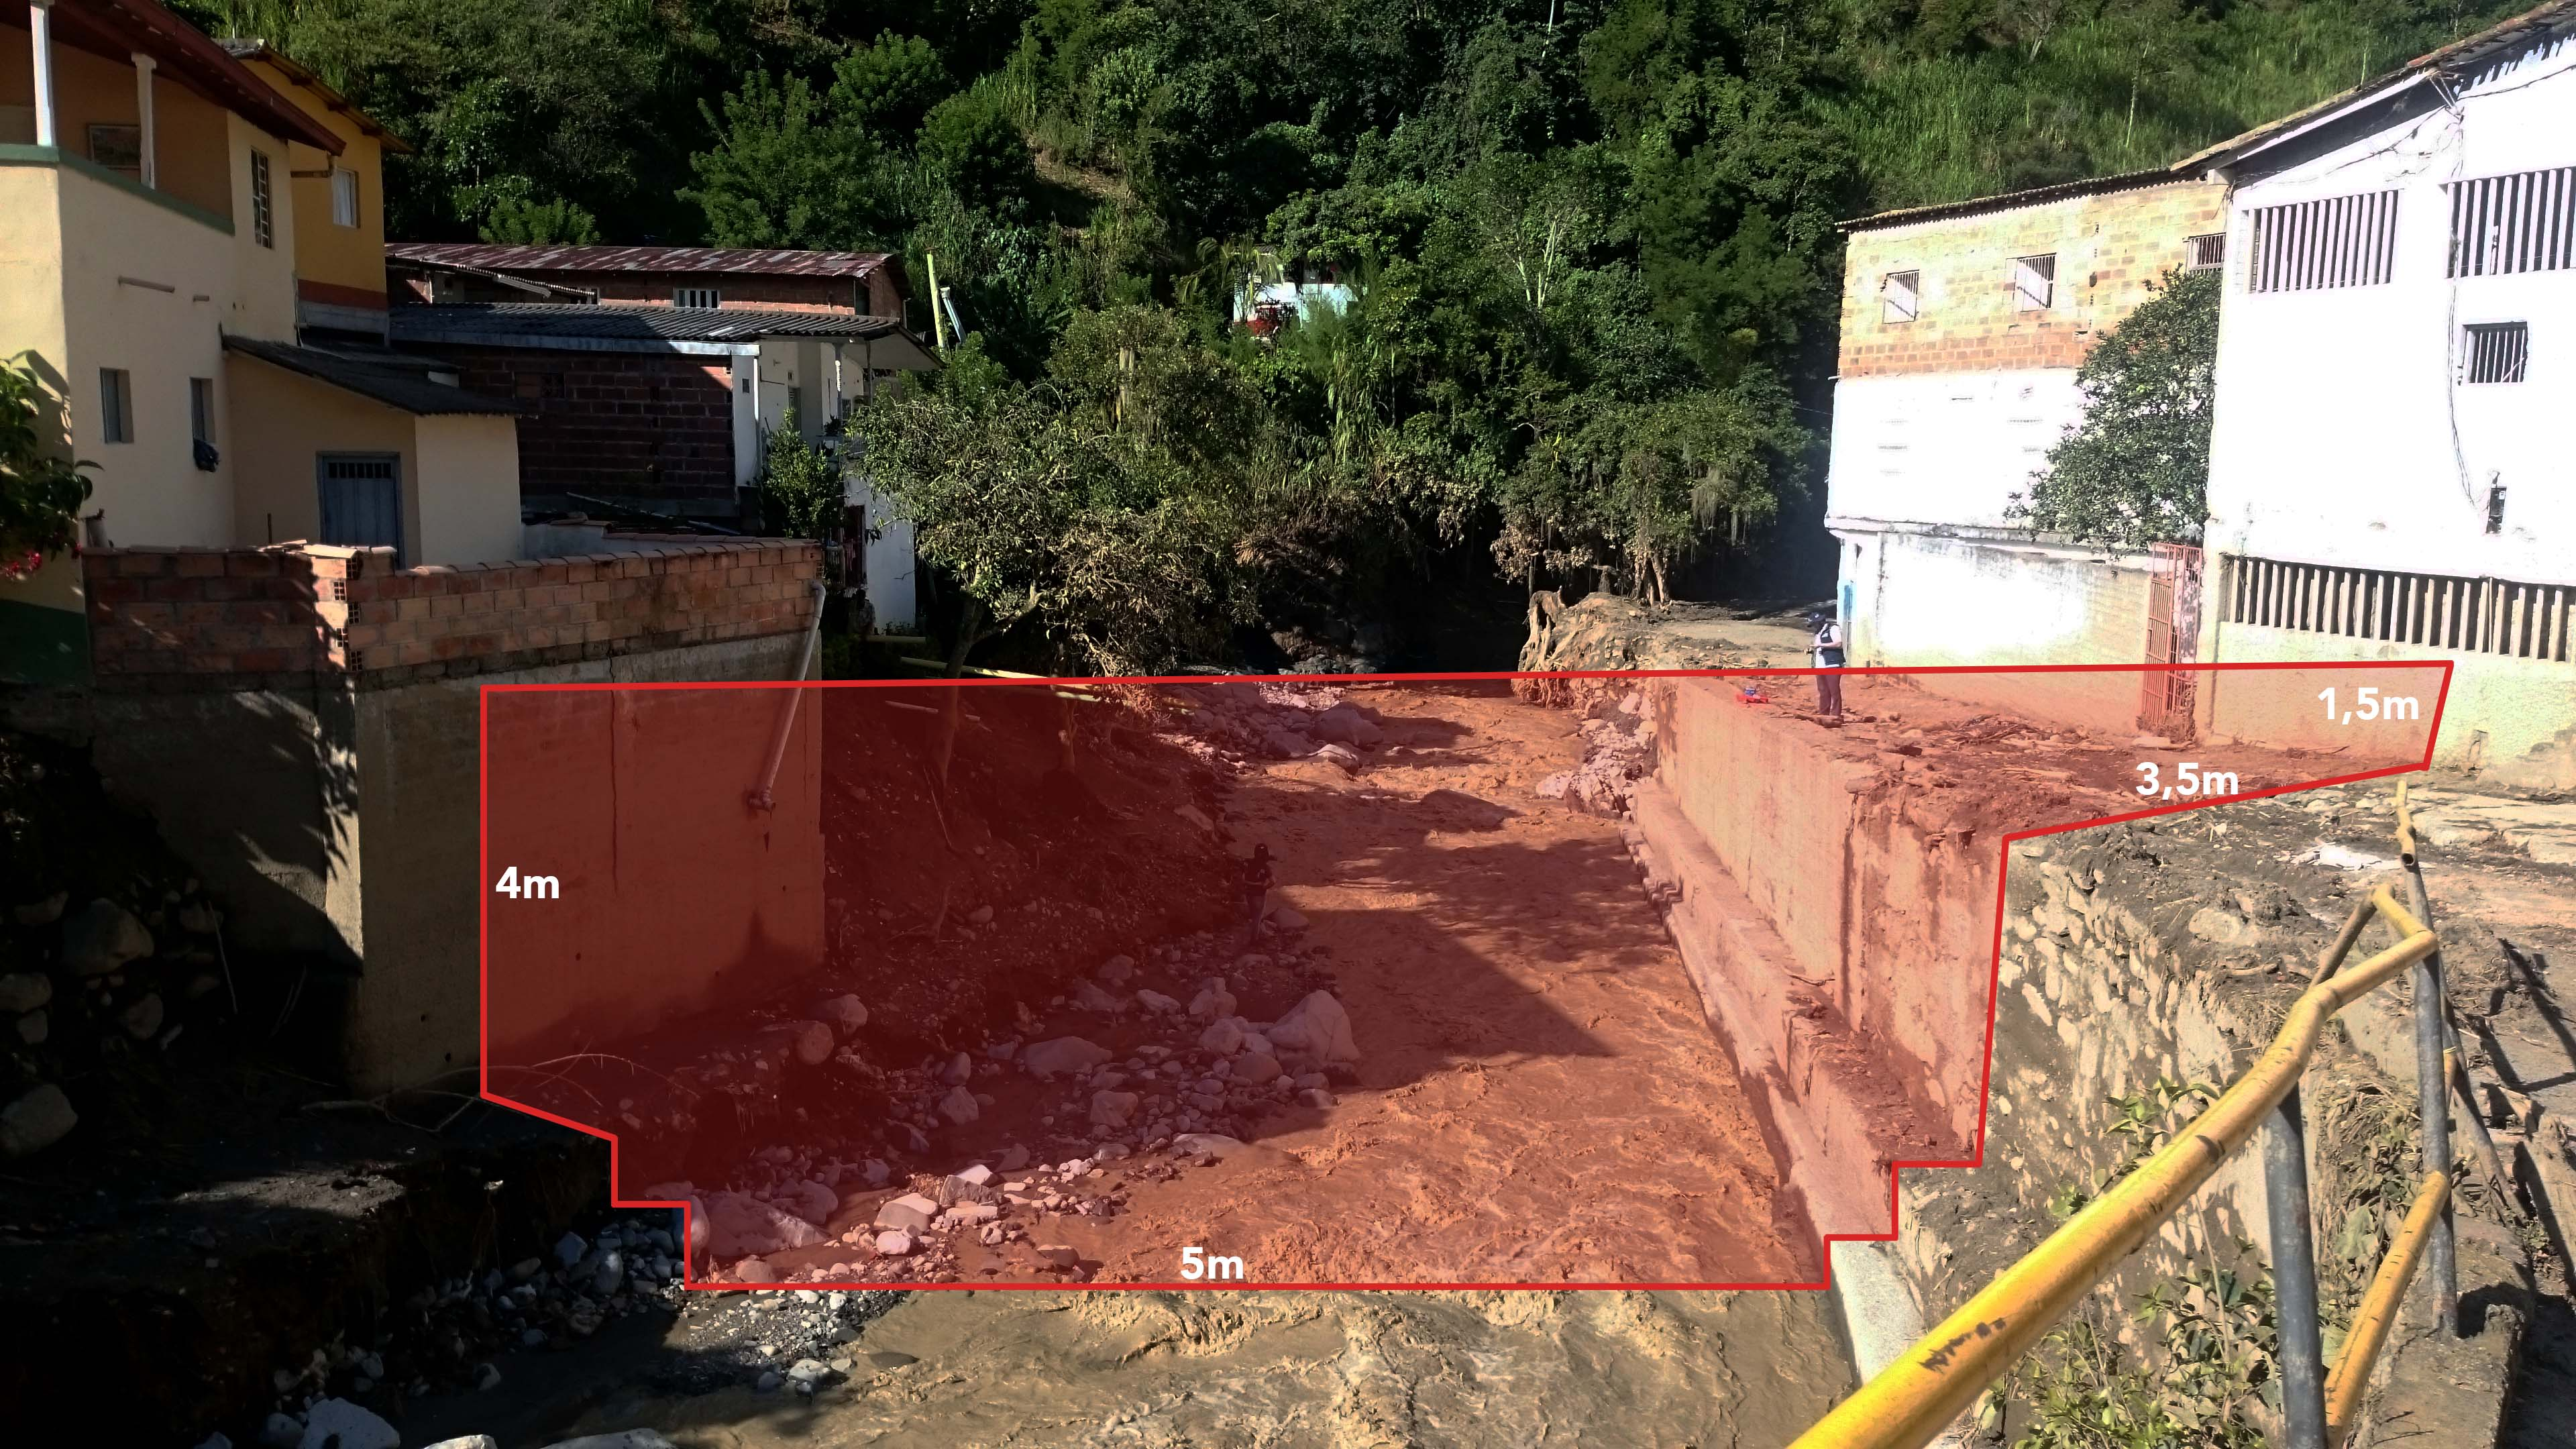
\includegraphics[width=8.3cm]{Figures/Salgar_SeccionAguasAbajo.jpg}
    \caption{Channel cross-section shown an example of flooded infrastructure after the flash flood event. The section shows mud marks on the walls with heights varying between 0.5 and 1.2 \DIFdelbeginFL \DIFdelFL{$m$}\DIFdelendFL \DIFaddbeginFL \DIFaddFL{m}\DIFaddendFL . These mud stains are evident in buildings located 4-5 \DIFdelbeginFL \DIFdelFL{$m$ }\DIFdelendFL \DIFaddbeginFL \DIFaddFL{m }\DIFaddendFL away from the channel. The photograph also shows the width of the channel and the total estimated depth during the flash flood.}
    \label{fig:Seccion}
\end{figure}

\DIFdelbegin \DIFdel{The reconstruction }\DIFdelend \DIFaddbegin \subsection{\DIFadd{Rainfall Information}}

\DIFadd{The assessment }\DIFaddend of the 2015 Salgar flash flood event following a hydrological modeling strategy uses a radar-based QPE technique developed by Sepúlveda and Hoyos (\DIFdelbegin \DIFdel{2018) }\DIFdelend \DIFaddbegin \DIFadd{2019) using rainfall gauges and disdrometers within the radar domain }\DIFaddend to obtain spatiotemporal precipitation maps over the basin. A detailed description of the \DIFaddbegin \DIFadd{rainfall }\DIFaddend estimation, as well as the overall meteorological conditions that led to the La Liboriana extreme event, are described in a companion paper (Hoyos et al. \DIFdelbegin \DIFdel{2018}\DIFdelend \DIFaddbegin \DIFadd{2019}\DIFaddend ). The QPE technique uses retrievals from a C-band polarimetric Doppler weather radar operated by the Sistema de \DIFdelbegin \DIFdel{Alertas Tempranas }\DIFdelend \DIFaddbegin \DIFadd{Alerta Temprana }\DIFaddend de Medellín y \DIFdelbegin \DIFdel{del }\DIFdelend \DIFaddbegin \DIFadd{el }\DIFaddend Valle de Aburra (SIATA, \DIFdelbegin \DIFdel{is }\DIFdelend a local early warning system from a neighboring region,  www.siata.gov.co)\DIFdelbegin \DIFdel{and it is located at 100$km$ }\DIFdelend \DIFaddbegin \DIFadd{, located around 90 $\text{km}$ }\DIFaddend away from the basin. The radar has an optimal optimum range of 120 \DIFdelbegin \DIFdel{$km$ radius }\DIFdelend \DIFaddbegin \DIFadd{$\text{km}$ radius for rainfall estimation }\DIFaddend and a maximum operational range of 240 \DIFdelbegin \DIFdel{$km$}\DIFdelend \DIFaddbegin \DIFadd{$\text{km}$ for weather detection}\DIFaddend . The radar operating strategy allows obtaining precipitation information every 5 \DIFdelbegin \DIFdel{$min$ and the }\DIFdelend \DIFaddbegin \DIFadd{minutes with a }\DIFaddend spatial resolution is about 128 \DIFdelbegin \DIFdel{$m$. The sensor is a C-band polarimetric Doppler weather radar operated by the Sistema de Alertas Tempranas de Medellín y del Valle de Aburra (SIATA, a local early warning system from a neighboring region, www.siata. gov.co)}\DIFdelend \DIFaddbegin \DIFadd{$\text{m}$. The results of the radar QPE methodology indicate that the rainfall estimation works well within a radius of 120km. Despite the distance between the radar and the basin, and the mountains between them, there are no blind spots for the radar. A  comparison between the radar QPE estimates and records from two rain gauges installed three days after the flash flood event show a correlation for an hourly time scale of 0.65. In addition to the rainfall quantification, radar retrievals, before feeding the hydrologic model,  are classified in convective and stratiform areas following a methodology proposed by \mbox{%DIFAUXCMD
\citet{Houze2015} }\hspace{0pt}%DIFAUXCMD
and \mbox{%DIFAUXCMD
\citet{Steiner1995}}\hspace{0pt}%DIFAUXCMD
.}\\

\DIFadd{Between May 15th and May 18th, 2015, several storms took place over La Liboriana basin.  During the night of May 17th, between 02:00 }\DIFaddend and \DIFdelbegin \DIFdel{located at 100$km$ away from the basin}\DIFdelend \DIFaddbegin \DIFadd{09:00 a.m. (local time), a precipitation event covered almost all the basin (hereafter referred to as precipitation Event 1).  Twenty hours later, between 23:00 p.m. of May 17 and 02:00 a.m. of May 18 two successive extreme convective systems occurred over the basin with the maximum intensity in the upper hills (precipitation Event 2).  Event 1 corresponds mainly to a stratiform event, covering almost all the basin area and with an average precipitation accumulation of 47 $\text{mm}$. Event 2 accumulated, in average over the basin, around 38 $\text{mm}$, however over the upper watershed the accumulation exceeded 180 $\text{mm}$. Figure \ref{fig:separacionLluvia}a presents the temporal evolution of the convective-stratiform rainfall partitioning during both Events 1 and 2. The main difference between both events is the timing of the convective versus stratiform participation within each case. Event 1 started as a stratiform precipitation event moving from the southwest, from the Department of Chocó to the Department of Antioquia across westernmost Andes mountain range}\DIFaddend . \DIFdelbegin \DIFdel{The radar has an optimal optimum rangeof 120 $km$ radius and a maximum operational range of 240 $km$. The radar operating strategy allows obtaining precipitation information every 5$min$ and with a spatial resolution is about 128 $m$}\DIFdelend \DIFaddbegin \DIFadd{Chochó is the rainiest department in Colombia, and one of the wettest places on Earth, due to the inflow of moisture from the Pacific Ocean and the orientation of the Andes mountain range \mbox{%DIFAUXCMD
\citep{poveda2000, Mapes2003}}\hspace{0pt}%DIFAUXCMD
.  After 3 hours of stratiform rainfall, training convective cores move over La Liboriana basin generating intense precipitation peaks during 2.5 hours. It is important to note that these cores did not strengthen within La Liboriana basin; these systems formed and intensified over the western hills of Farallones de Citará draining to the Department of Chocó towards the Atrato river. The latter is not a minor fact because once the convective system moved with a northeast direction, the maximum intensity cores did not fall over the steepest hills of La Liboriana basin but rather near the basin outlet where the slopes are considerably flatter. Figure \ref{fig:separacionLluvia}b shows the spatial distribution cumulative rainfall during Event 1, with the maximum precipitation located towards the bottom third of the basin. Event 2, on the other hand, started as a thunderstorm training event with two convective cores moving from the southeast followed by remaining stratiform precipitation.  Even though the average cumulative rainfall over the basin was 9 mm less than during Event 1, this event is characterized by orographic intensification within the basin leading to a more heterogeneous spatial distribution and with the highest cumulative precipitation in the steepest portion of the basin (see Figure \ref{fig:separacionLluvia}b). Event 2 spatial distribution and highly localized observed intensities most likely led to the flash-flooding episode, as it is explored in this work}\DIFaddend . \\

%DIF < %-----------------------------------------------------------
%DIF < %-----------------------------------------------------------
%DIF < Methodology
%DIF < %-----------------------------------------------------------
%DIF < %-----------------------------------------------------------
\DIFdelbegin \section{\DIFdel{Methodology}}
%DIFAUXCMD
\addtocounter{section}{-1}%DIFAUXCMD
%DIFDELCMD < \label{sec:methods}
%DIFDELCMD < %%%
\DIFdelend \DIFaddbegin \begin{figure}[t]
\centering
 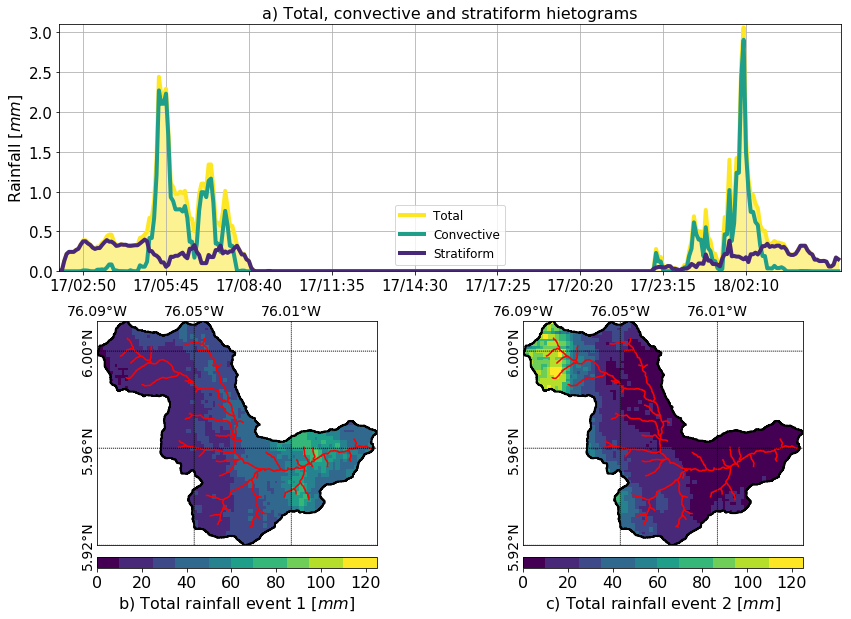
\includegraphics[width=12cm]{Figures/Rainfall_separation.png}
 \caption{\DIFaddFL{a) Temporal evolution of the convective-stratiform rainfall partitioning during both Events 1 and 2. The figure shows the total rainfall (yellow), and the convective (blue) and stratiform (green) portions integrated over La Liboriana basin. b) and c) Spatial distribution of the cumulative rainfall during Events 1 and 2 over La Liboriana basin.}}
    \label{fig:separacionLluvia}
\end{figure}
\DIFaddend 

The \DIFaddbegin \DIFadd{data requirements, and rainfall preprocessing needed for the }\DIFaddend overall methodology followed in the reconstruction of the 2015 Salgar flash flood \DIFdelbegin \DIFdel{, is presented in an illustrative }\DIFdelend \DIFaddbegin \DIFadd{are summarized in Table \ref{tab:data} and are   presented in a schematic }\DIFaddend diagram in Figure \ref{fig:EsquemaMetodologico}. \DIFaddbegin \\


    \begin{table}[]
        \centering
        \begin{tabularx}{\textwidth}{p{2.5cm} p{4cm} p{2cm} p{4cm} }
    \hline 
    \DIFaddFL{Item }& \DIFaddFL{Description }& \DIFaddFL{Period }& \DIFaddFL{Usage }\\
    \hline
\DIFaddFL{Radar data }& \DIFaddFL{QPE rainfall estimations }& \DIFaddFL{2015-05-17 to 2015-05-18 }& \DIFaddFL{Hydrologic model runs. Rainfall characterization and event analysis. }\\
\DIFaddFL{Field campaign }& \DIFaddFL{Maximum streamflow estimation trough visual inspection }& \DIFaddFL{2015-05-20 }& \DIFaddFL{Hydrologic model comparison for indirect validation. }\\
\DIFaddFL{Satellite imagery }& \DIFaddFL{Visible channel compositions from the Digital Globe CNES imagery }& \DIFaddFL{2015-05 (post-event) }& \DIFaddFL{Flash flood model validation, shallow land-slides model validation, and comparison with pre-event conditions. }\\
\DIFaddFL{Aerial photos }& \DIFaddFL{Aerial photos taken by the government of Antioquia during 2012. }& \DIFaddFL{2012 }& \DIFaddFL{Pre-event conditions comparison. }\\
\DIFaddFL{Soils description }& \DIFaddFL{Physical description of the soils of the region by \mbox{%DIFAUXCMD
\cite{Osorio2008} }\hspace{0pt}%DIFAUXCMD
}& \DIFaddFL{2008 }& \DIFaddFL{Hydrologic model setup. }\\
\hline
\end{tabularx}
        \caption{\DIFaddFL{Summary of the data used for the model setup.}}
        \label{tab:data}
    \end{table}

\begin{figure}[t]
\centering
 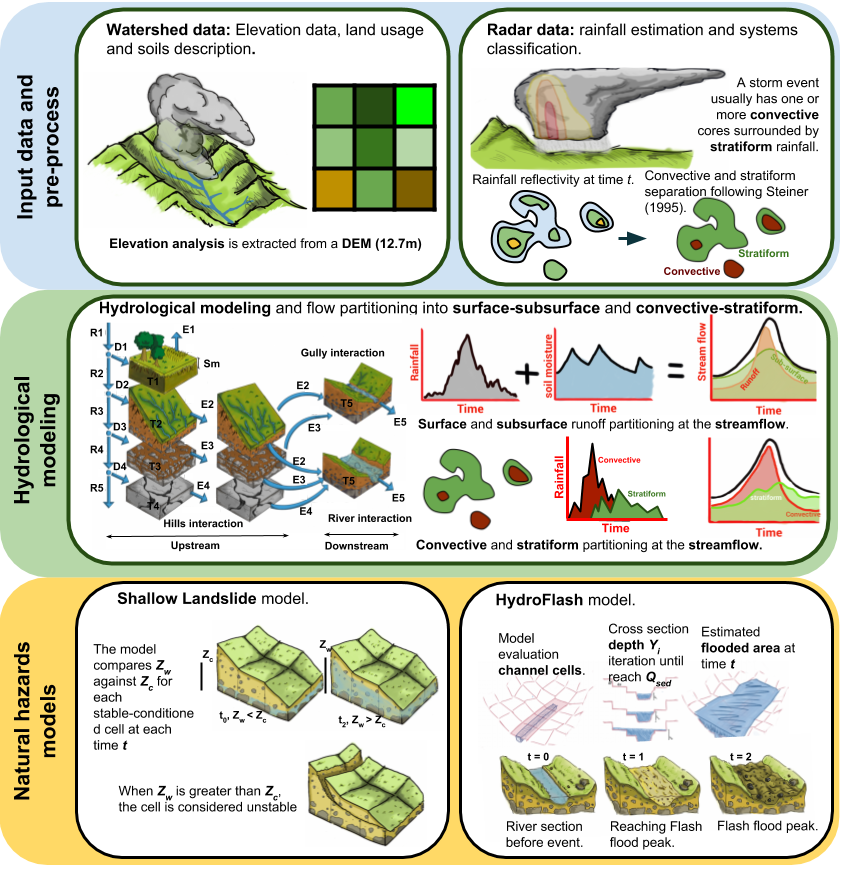
\includegraphics[width=12cm]{Figures/Salgar_Esquema_v2.png}
 \caption{\DIFaddFL{Illustrative diagram of the methodology followed in the present study. The top row represents the availability of a detailed DEM and  radar-based QPE as the basis of the modeling framework. The second row represents the mains aspects of the distributed hydrologic model used. In each cell five tanks represent the hydrological processes including capillary (tank 1), gravitational (tank 2), runoff (tank 3), baseflow (tank 4) and channel storage (tank 5).  The state of each tank varies in function of vertical and lateral flows as shown in the diagram, where the storage is represented by $S_i$, the vertical input by $D_i$ which in turns depends on the vertical flow through tanks $R_i$. $E_i$ represents the downstream connection between cells, and evaporation. The implementation of convective and stratiform rainfall separation and virtual tracers is also portrayed. The implementation of the shallow landslides model and HydroFlash are schematized in the bottom row.}}
    \label{fig:EsquemaMetodologico}
\end{figure}



%DIF > %-----------------------------------------------------------
%DIF > %-----------------------------------------------------------
%DIF > Methodology
%DIF > %-----------------------------------------------------------
%DIF > %-----------------------------------------------------------
\section{\DIFadd{Methodology}}
\label{sec:methods}

\subsection{\DIFadd{Hydrological modeling framework}}

\DIFaddend The availability of radar-based QPE and a detailed DEM allows the use of a modeling framework based on the distributed \DIFdelbegin \DIFdel{hydrological }\DIFdelend \DIFaddbegin \DIFadd{hydrologic }\DIFaddend model described in \citet{Velez2001} and \citet{Frances2007b} with important modifications\DIFdelbegin \DIFdel{(left column in Figure \ref{fig:EsquemaMetodologico}). The hydrological }\DIFdelend \DIFaddbegin \DIFadd{. The hydrologic }\DIFaddend model simulates different hydrological processes as independent, but interacting storages \DIFaddbegin \DIFadd{(second row, left panel in Figure \ref{fig:EsquemaMetodologico})}\DIFaddend .  The model distributes processes by cells; in each cell, five tanks represent the hydrological processes including capillary (tank 1), gravitational (tank 2), runoff (tank 3), baseflow (tank 4) and channel storage (tank 5).  The state of each tank varies in function of vertical and lateral flows as shown in the diagram, where the storage is represented by $S_i$, the vertical input \DIFaddbegin \DIFadd{to each tank }\DIFaddend by $D_i$\DIFaddbegin \DIFadd{, }\DIFaddend which in turns depends on \DIFaddbegin \DIFadd{the vertical flow through tanks }\DIFaddend $R_i$. $E_i$ represents the downstream connection between cells, except for tank 1, where $E_1$ represents the evaporation rate. Vertical flows are only time dependent, while lateral flows could also depend on the actual state of the tank (kinematic approximation).\\

\DIFdelbegin %DIFDELCMD < \begin{figure}[t]
%DIFDELCMD < \centering
%DIFDELCMD <  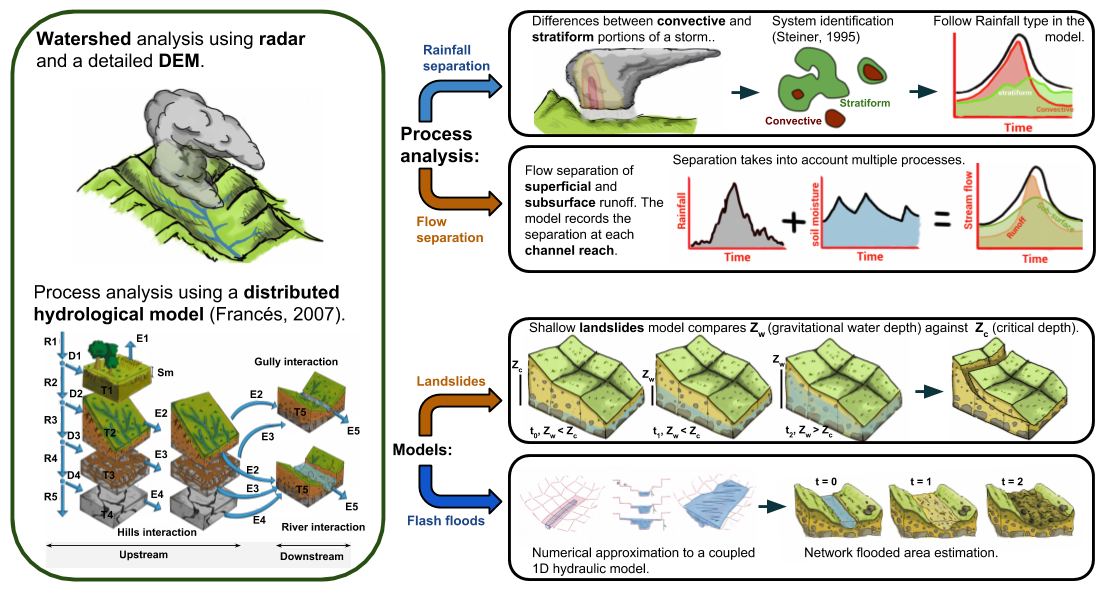
\includegraphics[width=12cm]{Figures/Salgar_Esquema_Metodologico.jpg}
%DIFDELCMD <  %%%
%DIFDELCMD < \caption{%
{%DIFAUXCMD
\DIFdelFL{Illustrative diagram of the methodology followed in the present study. The left column represents the availability of radar-based QPE and a detailed DEM as the basis of the modeling framework and the mains aspects of the distributed hydrological model used. In each cell five tanks represent the hydrological processes including capillary (tank 1), gravitational (tank 2), runoff (tank 3), baseflow (tank 4) and channel storage (tank 5).  The state of each tank varies in function of vertical and lateral flows as shown in the diagram, where the storage is represented by $S_i$, the vertical input by $D_i$ which in turns  depends on $R_i$. $E_i$ represents the downstream connection between cells, and evaporation. The implementation of convective and stratiform rainfall separation and virtual tracers are presented in the top two right panels. The implementation of the shallow landslides model and HydroFlash are schematized in the bottom two right panels.}}
    %DIFAUXCMD
%DIFDELCMD < \label{fig:EsquemaMetodologico}
%DIFDELCMD < \end{figure}
%DIFDELCMD < 

%DIFDELCMD < %%%
\DIFdelend The model modifications fall in four different categories: (i) the direct use of radar QPE as a source of rainfall information, (ii) the implementation of virtual tracers for surface and subsurface discharge  as well as for convective and stratiform water tracing,  (iii)  the \DIFdelbegin \DIFdel{development of two modules for hazard assessment, and (iv) the }\DIFdelend enforcement of a maximum gravitational storage ($H_{g}$) to allow Hortonian runoff (return flow from $S_3$ \DIFaddbegin \DIFadd{(tank 3) }\DIFaddend to $S_2$ \DIFdelbegin \DIFdel{). The virtual tracers are critical to explore separately the relative role of superficial runoff and subsurface flow, as well as the relative importance of convective and stratiform precipitation in flash flood generation. The convective and stratiform classification follows the methodology proposed by \mbox{%DIFAUXCMD
\citet{Houze2015} }\hspace{0pt}%DIFAUXCMD
and \mbox{%DIFAUXCMD
\citet{Steiner1995}}\hspace{0pt}%DIFAUXCMD
}\DIFdelend \DIFaddbegin \DIFadd{(tank 2)), and (iv)  the development of two modules for hazard assessment}\DIFaddend . The implementation of \DIFdelbegin \DIFdel{convective and stratiform rainfall separation and virtual tracers are presented }\DIFdelend \DIFaddbegin \DIFadd{virtual tracers is represented }\DIFaddend in the top two right panels of the \DIFdelbegin \DIFdel{illustrative }\DIFdelend diagram in Figure\ref{fig:EsquemaMetodologico}.\DIFdelbegin \DIFdel{The hydrological modelallows hazard assessment by coupling a  shallow landslide model\mbox{%DIFAUXCMD
\citep{Aristizabal2016}}\hspace{0pt}%DIFAUXCMD
, }\DIFdelend \DIFaddbegin \\

\subsubsection{\DIFadd{Hydrological runoff scheme modification}}

\DIFadd{In the model, horizontal flow equations could be either linear or potential, as shown in equation \ref{eq:generica}. In the modified hydrologic model, $\beta$ and $\alpha$ are estimated by the user and then set into the model. In the non-lineal approximation $\beta$ is a coefficient that summarizes local properties invariant over time, like the slope or the hydraulic conductivity. $\alpha$ is an exponent that change in function of the adopted approximation. From equations \ref{eq:generica} to \ref{eq:kubota}, $A_i(t)$ corresponds to the sectional area of each storage, $A_i(t)$ vary in function of the tank storage $S_i(t)$ according to equation \ref{eq:balance}.
}

\begin{equation}
 \DIFadd{v_{tank}(t) = \beta A_i(t) ^{\alpha} 
    \label{eq:generica}
}\end{equation}

\DIFadd{Non-linear equations in lateral flows could result in a better representation of processes at high resolutions \mbox{%DIFAUXCMD
\citep{Beven1981, Kirkby1967}}\hspace{0pt}%DIFAUXCMD
.  A non-linear approximation to runoff is presented in equation \ref{eq:runoff}.   This approximation is a modification of Manning's formula for flow in gullies. According to \mbox{%DIFAUXCMD
\citet{Foster1984}}\hspace{0pt}%DIFAUXCMD
, $\varepsilon$ }\DIFaddend and \DIFdelbegin \DIFdel{a new low-cost 1d hydraulic flash flood model referred to here as }\textbf{\DIFdel{HydroFlash}}%DIFAUXCMD
\DIFdel{.
The implementation of }\DIFdelend \DIFaddbegin \DIFadd{$e_1$ are a coefficient and an exponent used to translate the manning channel concept into multiple small channels or gullies. The values of $\varepsilon$ and $e_1$ are 0.5 and 0.64, respectively \mbox{%DIFAUXCMD
\citep{Foster1984}}\hspace{0pt}%DIFAUXCMD
. $A_2$ is the corresponding sectional area obtained from $S_2$ by using the equation (\ref{eq:balance}). And $S_0$ is the slope of the cell.    
}

\DIFadd{The non-linear equation \ref{eq:kubota} corresponds to an adaptation of \mbox{%DIFAUXCMD
\citet{Kubota1995} }\hspace{0pt}%DIFAUXCMD
formula for subsurface runoff where $k_s$ is the saturated hydraulic conductivity, and the exponent $b$ is dependent on the soil type, assumed equal to 2.  $A_g$ is the equivalent cross-section area to the maximum gravitational storage ($H_g$).  $A_3$ is the corresponding sectional area of the gravitational storage ($S_3$) obtained by using equation (\ref{eq:balance}).  There is also return flow from tank 3 to tank 2 when $S_3=H_g$, representing runoff generation by saturation.   
}

\begin{equation}
 \DIFadd{v_{2} = \frac{\varepsilon}{n}  S_{0}^{1/2} A_{2}(t)^{(2/3) e_1}
    \label{eq:runoff}
}\end{equation}
\begin{equation}
 \DIFadd{v_3 = \frac{K_s S_{o}^{2}}{(b+1) A_{g}^{b}} A_{3}(t)^{b}
    \label{eq:kubota}
}\end{equation}

\DIFadd{The equations describe the momentum of a kinematic wave approximation. In both cases, velocity depends on the tank storage. These relations are summarized in equation \ref{eq:generica},  that could be solved numerically coupled with a mass balance equation (equation \ref{eq:balance}). This equation takes into account the storage at each time step ($S_{tank}(t)$), the longitude of the element ($\Delta x$), the time step size ($\Delta t$), and the speed estimated for the flow in the time step ($v_{tank}(t)$).  Equation \ref{eq:balance} is related to equation \ref{eq:generica} through the velocity term for that tank ($v_{tank}$) and }\DIFaddend the \DIFdelbegin \DIFdel{shallow landslides model and HydroFlash are schematized in the bottom two right panels of the illustrative diagram in Figure \ref{fig:EsquemaMetodologico}.    
}%DIFDELCMD < \\
%DIFDELCMD < %%%
\DIFdelend \DIFaddbegin \DIFadd{cross-sectional area of the tank ($A_{tank}$).  The solution to $v_{tank}$ and $A_{tank}$ is obtained through an iterative scheme.  The total outflow from the tank is calculated using equation \ref{eq:volSalida}.
}\DIFaddend 

\DIFdelbegin \DIFdel{For the technically inclined reader, the hydrological model and sub-models are written in Fortran 90,  and the interface to the model, pre-process, and post-process tools are in python 2.7.  The Fortran code is warped to python using }\textbf{\DIFdel{f2py}} %DIFAUXCMD
\DIFdel{\mbox{%DIFAUXCMD
\citep{Peterson2009} }\hspace{0pt}%DIFAUXCMD
and it is publicly available under the Watershed Modelling Framework }\textbf{\DIFdel{WMF}} %DIFAUXCMD
\DIFdel{in a web repository (}%DIFDELCMD < \href{https://github.com/nicolas998/WMF.git}{\textbf{GitHub}}%%%
\DIFdel{).  }%DIFDELCMD < \\
%DIFDELCMD < %%%
\DIFdelend \DIFaddbegin \begin{equation}
 \DIFadd{A_i(t) = \frac{S_{tank}(t)}{\Delta x + v_{tank}(t) \Delta t}
    \label{eq:balance}
}\end{equation}
\begin{equation}
    \DIFadd{E_{tank}(t) =  A_{tank}(t) v_{tank}(t) \Delta t
     \label{eq:volSalida}
}\end{equation}
\DIFaddend 

\DIFdelbegin \subsection{\DIFdel{Virtual Tracers}}
%DIFAUXCMD
\addtocounter{subsection}{-1}%DIFAUXCMD
\DIFdelend \DIFaddbegin \subsubsection{\DIFadd{Virtual Tracers}}
\DIFaddend 

Virtual tracers are implemented into the model to discriminate streamflow source in superficial runoff and subsurface flow and to assess the portion of streamflow from convective rainfall and stratiform precipitation, recording at each time stem and each cell the source of water.  The model archives the results of the virtual tracing algorithm at the outlet of the basin and at each reach allowing the study of the role of flows from different nature during extreme events at different spatial scales to get more insights about the soil-driven flow regulation. \DIFdelbegin \DIFdel{The soil texture and composition could play diverging roles during extreme events. The soil could work as a porous medium in which the water travels fast, making the subsurface flow an essential part of the hydrograph, or on the other hand, its saturation could lead to a decrease in infiltration rates and a potential increase of surface runoff generation.}\DIFdelend \\

The flow separation module operates in tanks 2 (runoff storage) and 3 (subsurface storage).  The module marks water once it reaches any of those two tanks and the runoff-subsurface flow percentage are taken into account once the water enters tank 5 (the channel).   At this point, the scheme assumes that the water in the channel is well mixed,  implying that the flow percentage is constant until a new inflow enters the channel.\\

\DIFdelbegin \DIFdel{Both spatial and temporal rainfall variability influence the hydrograph \mbox{%DIFAUXCMD
\citet{Shope2016}}\hspace{0pt}%DIFAUXCMD
. Stratiform rain cells cover large areas and are related to long duration hydrographs with low peak flow.  On the other hand, convective rainfall cells cover limited areas and are related to short duration hydrographs with high peak flows.  Stratiform rainfall tends to recharge the basin, while convective tends to increase runoff generation and the formation of the hydrograph.  In the literature, these associations have often been more qualitative than quantitative \mbox{%DIFAUXCMD
\citep{Creutin2003a,Salek2006,Borga2014}}\hspace{0pt}%DIFAUXCMD
.}%DIFDELCMD < \\
%DIFDELCMD < 

%DIFDELCMD < %%%
\DIFdel{Rainfall from radar reflectivity fields is classified into stratiform and convective using the \mbox{%DIFAUXCMD
\cite{Steiner1995} }\hspace{0pt}%DIFAUXCMD
approach before the implementation of the rainfalltracer.  At }\DIFdelend \DIFaddbegin \DIFadd{With a similar concept, the model also follows convective and stratiform rainfall.  For this, at }\DIFaddend each time step, the model takes into account the \DIFdelbegin \DIFdel{total rainfall , assuming }\DIFdelend \DIFaddbegin \DIFadd{rainfall classified as convective or stratiform, and assumes }\DIFaddend that at each particular cell the precipitation is either entirely convective or entirely stratiform. This assumption could lead to estimation errors at basins represented by coarse cells (low DEM resolution) where convective and stratiform precipitation are likely to coexist. In the present study the spatial resolution of the DEM is 12.7$m$, higher than the resolution of the radar retrievals (about 125$m$), so the potential convective and stratiform rainfall concurrence is very low, and it could not be identified using the \cite{Steiner1995} approach.\DIFdelbegin \DIFdel{Once within the model, rainfall separation follows the methodology proposed for flow type separation.}\DIFdelend \\

\DIFdelbegin \subsection{\DIFdel{Hazards Assessment}}
%DIFAUXCMD
\addtocounter{subsection}{-1}%DIFAUXCMD
\DIFdelend \DIFaddbegin \subsubsection{\DIFadd{Hydrologic model calibration}}
\DIFaddend 

\DIFdelbegin \DIFdel{During the 2015 La Liboriana flash flood event, two central processes took place.  Shallow landslides occurred in the upper basin , and a flash flood generated flooding, and human and infrastructure losses.}\DIFdelend \DIFaddbegin \DIFadd{The hydrologic model requires a total of ten parameters. Table \ref{tab:parameters} includes all the parameters used in the model.  The values of the parameters were derived from the soil properties described in section 2. Due to the lack of detailed information in the region, parameters such as the infiltration and percolation rates are assumed as constant in all the basin.  Other parameters such as the capillary and gravitational storage vary in function of geomorphological characteristics of the basin such as the elevation and slope. According to \mbox{%DIFAUXCMD
\cite{Frances2007c}}\hspace{0pt}%DIFAUXCMD
, during the calibration process, each physical parameter is scaled by a constant value in the entire basin. Table \ref{tab:parameters} includes the mean value for all the parameters used in the model and the scalar value adjusted during the model calibration.
}

\begin{table}[]
        \centering
        \begin{tabularx}{\textwidth}{p{3cm} p{2.2cm} p{1.5cm} p{2cm} p{3.5cm}}
\hline
\DIFaddFL{Parameter Name }& \DIFaddFL{Symbol }& \DIFaddFL{Scalar Parameter }& \DIFaddFL{Mean Value }& \DIFaddFL{Spatial distribution }\DIFaddendFL \\
\DIFaddbeginFL \hline
\DIFaddFL{Capilary storge }& \DIFaddFL{Hu }[\DIFaddFL{mm}] & \DIFaddFL{1 }& \DIFaddFL{39 }& \DIFaddFL{In function of the slope }\\
\DIFaddFL{Gravitational storage }& \DIFaddFL{Hg }[\DIFaddFL{mm}] & \DIFaddFL{1 }& \DIFaddFL{34 }& \DIFaddFL{As a function of the slope }\\
\DIFaddFL{Evaporation rate }& \DIFaddFL{Etr }[\DIFaddFL{mm/s}] & \DIFaddFL{0.1 }& \DIFaddFL{0.01 }& \DIFaddFL{As a function of the DEM }\\
\DIFaddFL{Infiltration rate }& \DIFaddFL{ks }[\DIFaddFL{mm/s}] & \DIFaddFL{2.7 }& \DIFaddFL{0.0012 }& \DIFaddFL{Lumped }\\
\DIFaddFL{Percolation rate }& \DIFaddFL{kp }[\DIFaddFL{mm/s}] & \DIFaddFL{0.8 }& \DIFaddFL{0.00012 }& \DIFaddFL{Lumped }\\
\DIFaddFL{System losess }& \DIFaddFL{Kf }[\DIFaddFL{mm/s}] & \DIFaddFL{0 }& \DIFaddFL{0.0 }& \DIFaddFL{Lumped }\\
\DIFaddFL{Surface speed }& \DIFaddFL{vr }[\DIFaddFL{m/s}] & \DIFaddFL{0.5 }& \DIFaddFL{6.4 }& \DIFaddFL{As a function of the slope and storage }\\
\DIFaddFL{Subsurface speed }& \DIFaddFL{vs }[\DIFaddFL{m/s}] & \DIFaddFL{1 }& \DIFaddFL{7.1 }& \DIFaddFL{As a function of the slope, Hg and storage}\\
\DIFaddFL{Subterranean speed }& \DIFaddFL{vb }[\DIFaddFL{m/s}] & \DIFaddFL{0.5 }& \DIFaddFL{0.000095 }& \DIFaddFL{Lumped }\\
\DIFaddFL{Channel speed }& \DIFaddFL{vc }[\DIFaddFL{m/s}] & \DIFaddFL{1 }& \DIFaddFL{0.95 }& \DIFaddFL{As a function of the slope, acumulated area, and storage }\\
\hline
\end{tabularx}
        \caption{\DIFaddFL{Hydrologic model parameters.}}
        \label{tab:parameters}
    \end{table}
\DIFaddend 

\DIFdelbegin \subsubsection*{\DIFdel{Shallow landslides sub-model}}
%DIFAUXCMD
\DIFdelend \DIFaddbegin \subsection{\DIFadd{Shallow landslides sub-model}}
\DIFaddend 

The shallow landslides submodel coupled to the \DIFdelbegin \DIFdel{hydrological }\DIFdelend \DIFaddbegin \DIFadd{hydrologic }\DIFaddend model is proposed by  \citeauthor{Aristizabal2016}.  The \DIFdelbegin \DIFdel{model conceptualizes the stability of a cell based on the concept of an infinite slope described by the geomorphological and soil properties of the cell. The model }\DIFdelend \DIFaddbegin \DIFadd{submodel }\DIFaddend classifies cells into three groups: unconditionally stable, conditionally stable and unconditionally unstable. Figure \ref{fig:ModeloEstabilidad} describes the variables of the model and the balance of forces considered. Three parameters determine stability of each cell: (i) residual soil thickness water table $Z_{i,min}$ estimated as in equation \DIFdelbegin \DIFdel{(\ref{eq:zmin})}\DIFdelend \DIFaddbegin \DIFadd{\ref{eq:zmin}}\DIFaddend , (ii) the maximum soil depth at which a particular soil remains stable $Z_{i,max}$  estimated as in equation \DIFdelbegin \DIFdel{(\ref{eq:zmax})}\DIFdelend \DIFaddbegin \DIFadd{\ref{eq:zmax}}\DIFaddend , and (iii) the maximum slope at which the soil remains stable $\beta_{i,0}$ estimated as in equation \DIFdelbegin \DIFdel{(\ref{eq:bo}). }%DIFDELCMD < \\
%DIFDELCMD < 

%DIFDELCMD < \begin{figure}[t]
%DIFDELCMD < \centering
%DIFDELCMD <  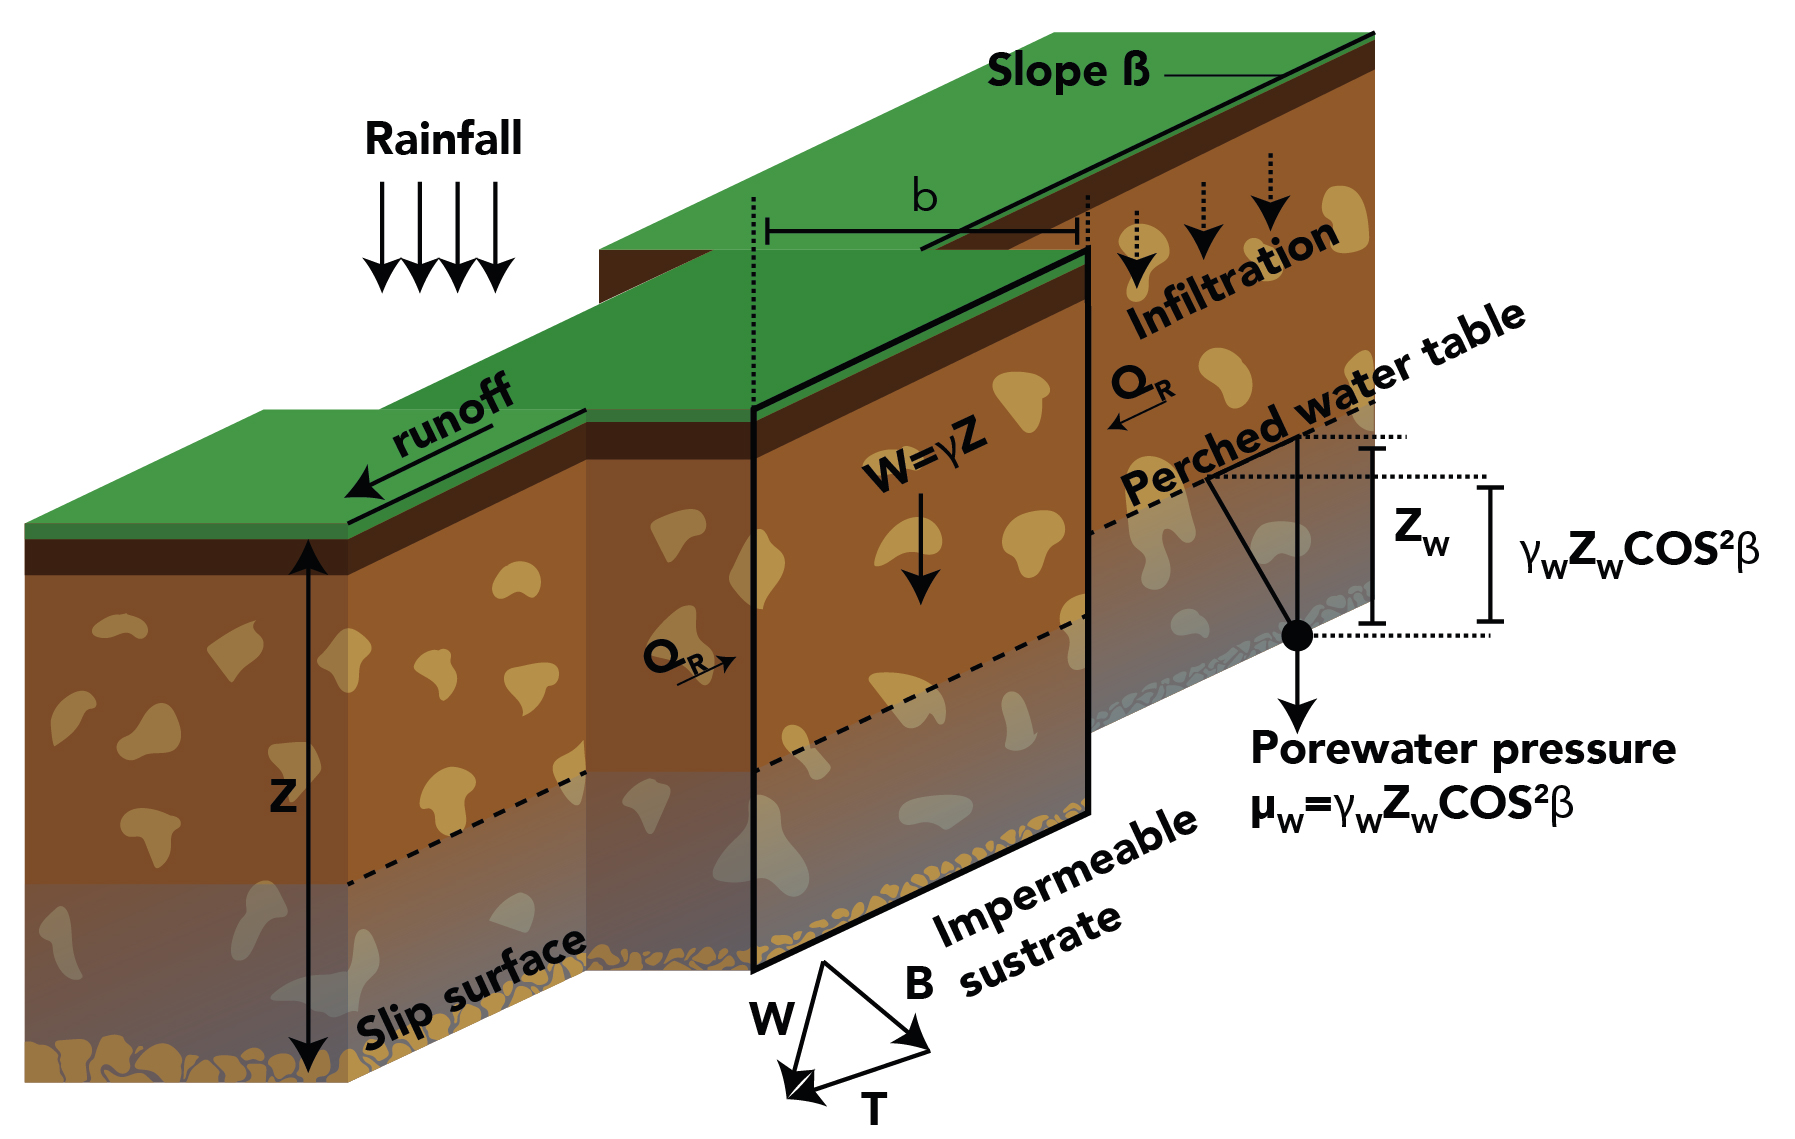
\includegraphics[width=8.3cm]{Figures/slides-escheme.jpg}
%DIFDELCMD <  \caption{%%%
\DIFdelFL{The geotechnical conceptual model}\DIFdelendFL \DIFaddbeginFL \DIFaddFL{\ref{eq:bo}}\DIFaddendFL . \DIFaddbeginFL \DIFaddFL{In the equations and in the Figure \ref{fig:ModeloEstabilidad} }\DIFaddendFL $\gamma$ \DIFdelbeginFL \DIFdelFL{is the soil bulk density, }\DIFdelendFL \DIFaddbeginFL \DIFaddFL{is the soil bulk density, }\DIFaddendFL $\gamma_w$ \DIFdelbeginFL \DIFdelFL{is the water density, }\DIFdelendFL \DIFaddbeginFL \DIFaddFL{is the water density, }\DIFaddendFL $Z_w$ \DIFdelbeginFL \DIFdelFL{is the saturated soil thickness above the slip surface, }\DIFdelendFL \DIFaddbeginFL \DIFaddFL{is the saturated soil thickness above the slip surface, }\DIFaddendFL $Z$ \DIFdelbeginFL \DIFdelFL{is the soil
thickness measured vertically, }\DIFdelendFL \DIFaddbeginFL \DIFaddFL{is the soil thickness measured vertically, }\DIFaddendFL $\beta$ \DIFdelbeginFL \DIFdelFL{is the gradient of the hillslope. And }\DIFdelendFL \DIFaddbeginFL \DIFaddFL{is the gradient of the hillslope, and $\phi$ is the soil stability angle. }\DIFaddendFL $Q_L$ and $Q_R$ \DIFdelbeginFL \DIFdelFL{are the resultant forces on the sides of the slice}\DIFdelendFL \DIFaddbeginFL \DIFaddFL{are the resultant forces on the sides of the slice.
}

\begin{figure}[t]
\centering
 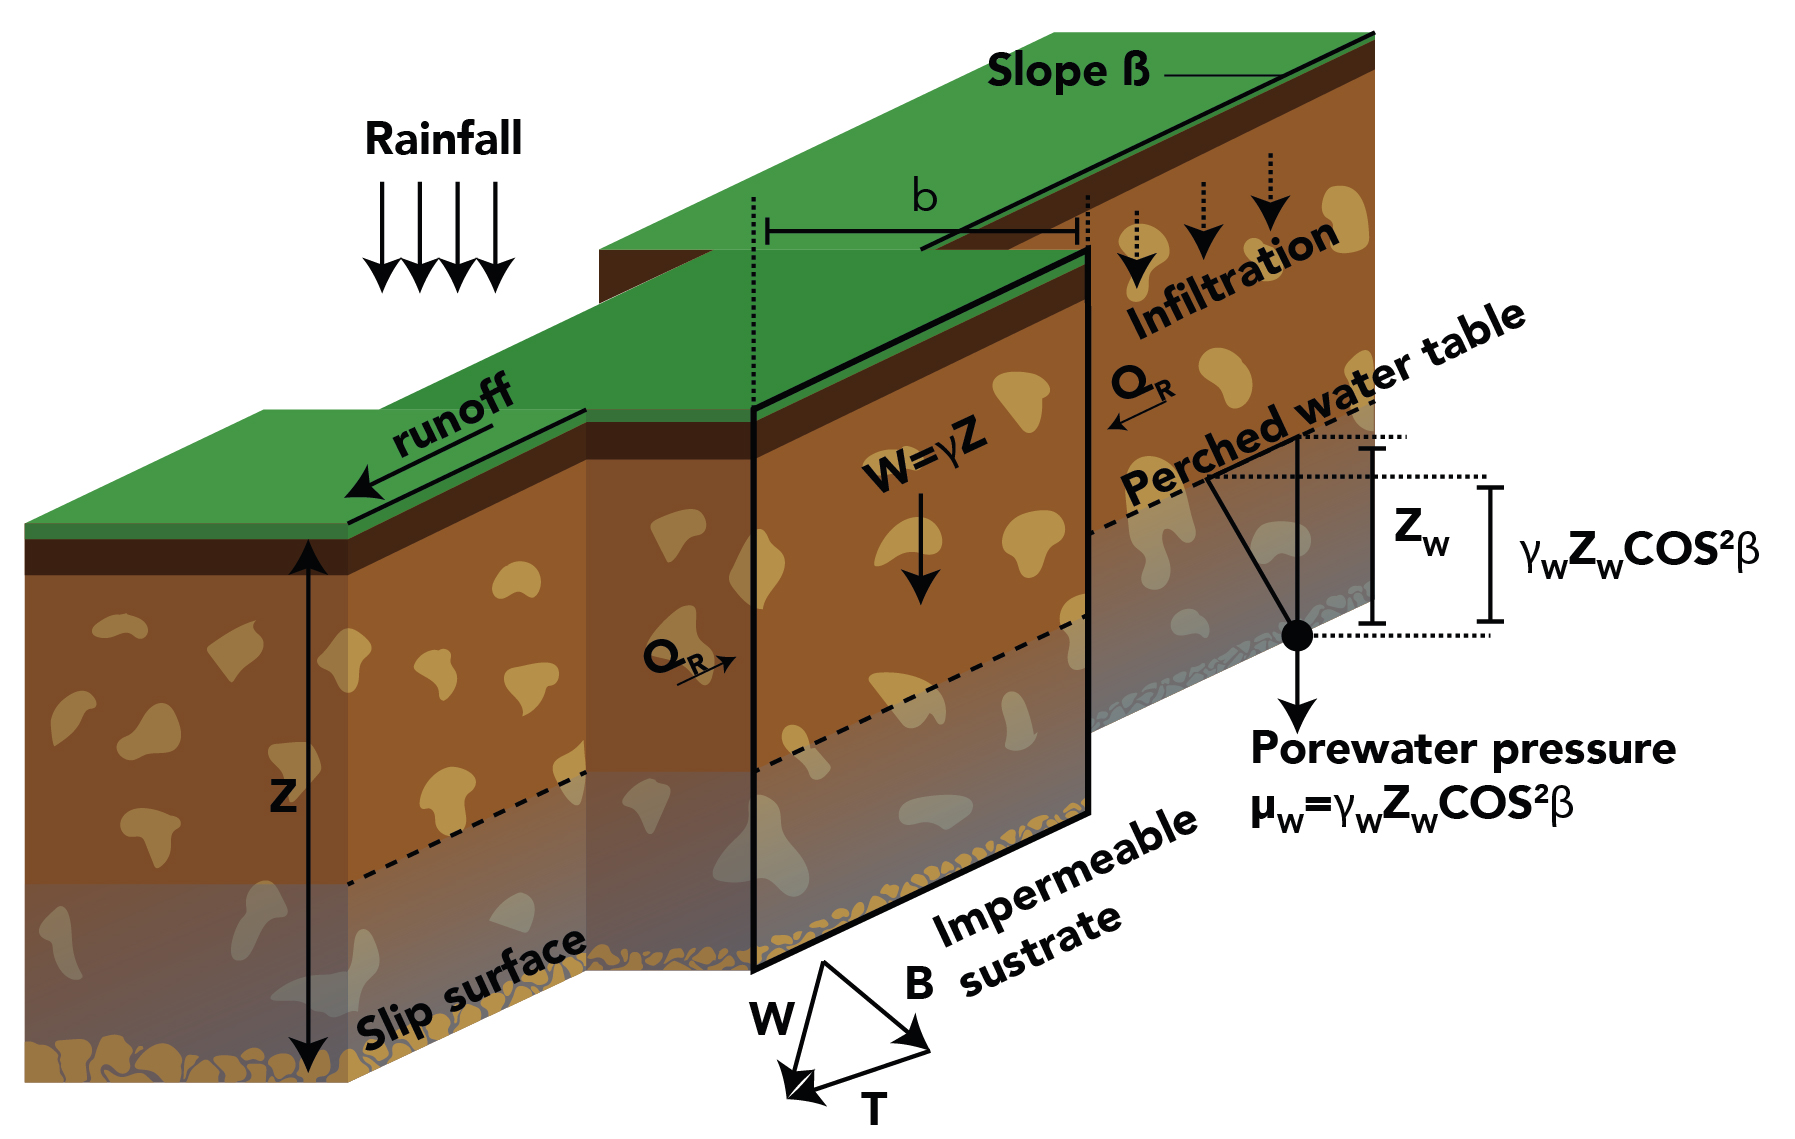
\includegraphics[width=8.3cm]{Figures/slides-escheme.jpg}
 \caption{\DIFaddFL{The geotechnical conceptual model}\DIFaddendFL . Figure and description are adapted from \citet{Aristizabal2016}.}
    \label{fig:ModeloEstabilidad}
\end{figure}

\begin{equation}
 Z_{i,min} = \frac{C^{'}}{\gamma_w cos^2 \beta tan \phi + \gamma cos^2 \beta (tan\beta - tan \phi)}
    \label{eq:zmin}
\end{equation}
\begin{equation}
 Z_{i,max} = \frac{C^{'}}{\gamma cos^2 \beta (tan\beta - tan \phi)}
 \label{eq:zmax}
\end{equation}
\begin{equation}
 \beta_{i,0} = tan ^{-1} \left[ tan \phi \left( 1- \frac{\gamma_w}{\gamma}\right) \right]
 \label{eq:bo}
\end{equation}

The model assess conditionally stable cells in function of their perched water table for each cell ($Z_{i,w}$, equation \DIFdelbegin \DIFdel{(\ref{eq:z}) }\DIFdelend \DIFaddbegin \DIFadd{\ref{eq:z}}\DIFaddend ) and the critical satured depth ($Z_{i,c}$\DIFaddbegin \DIFadd{, equation (\ref{eq:Zcrit})}\DIFaddend ).  Slope failure occurs when $Z_{i,w}$ is greater than $Z_{i,c}$. \DIFdelbegin \DIFdel{$Z_{i,c}$ is obtain using equation (\ref{eq:Zcrit}) .}%DIFDELCMD < \\
%DIFDELCMD < 

%DIFDELCMD < %%%
\begin{displaymath}
 \DIFdel{Z_{i,w}(t) = \frac{S_{3,t}}{W_c - W_{fc}}
 %DIFDELCMD < \label{eq:z}%%%
}\end{displaymath}
%DIFAUXCMD
\begin{displaymath}
 \DIFdel{Z_{i,c} = \frac{\gamma}{\gamma_w} Z \left( 1-\frac{tan \beta}{tan\phi} \right)
     + \frac{C^{'}}{\gamma_w cos^2 \beta tan\phi}
 %DIFDELCMD < \label{eq:Zcrit}%%%
}\end{displaymath}
%DIFAUXCMD
\DIFdel{where }\DIFdelend \DIFaddbegin \DIFadd{At equation (\ref{eq:z}) }\DIFaddend $S_{3,i}$ represents gravitational storage, $Ws$ and $W_{fc}$ the soil saturation and field capacity respectively\DIFdelbegin \DIFdel{,  $\gamma$ represents soil density, $\phi$ is the soil stability angle, }\DIFdelend \DIFaddbegin \DIFadd{. And in equation (\ref{eq:Zcrit}) }\DIFaddend $C^{'}$ \DIFaddbegin \DIFadd{represents }\DIFaddend the soil cohesion and $\beta$ the cell slope.

\DIFdelbegin \subsubsection*{\DIFdel{Flash flood submodel (HydroFlash)}}
%DIFAUXCMD
\DIFdelend \DIFaddbegin \begin{equation}
 \DIFadd{Z_{i,w}(t) = \frac{S_{3,t}}{W_c - W_{fc}}
 \label{eq:z}
}\end{equation}
\begin{equation}
 \DIFadd{Z_{i,c} = \frac{\gamma}{\gamma_w} Z \left( 1-\frac{tan \beta}{tan\phi} \right)
     + \frac{C^{'}}{\gamma_w cos^2 \beta tan\phi}
 \label{eq:Zcrit}
}\end{equation}

\subsection{\DIFadd{Flash flood submodel (HydroFlash)}}
\DIFaddend 

\DIFdelbegin \DIFdel{It is common to use complex hydraulic 2D and 3D models, such as Iber \mbox{%DIFAUXCMD
\citep{Cea2015} }\hspace{0pt}%DIFAUXCMD
or HEC \mbox{%DIFAUXCMD
\citep{Gibson2010} }\hspace{0pt}%DIFAUXCMD
for flood spots identification.  This kind of modeling requires detailed information about the terrain and river bathymetry and are usually implemented for a particular river cross section due to the high information demand and high computational costs,  precluding the operational implementation of 2D and 3D methodologies in regions with scarce resources.  Also, this traditional hydraulic methodology tends to analyze only some network elements, overlooking the complexity of the basin. }\DIFdelend In this work, we introduce a low-cost 1D hydraulic model for flash flood simulation referred to as HydroFlash. The model extracts the cross-profile from the DEM  for each cell considered part of the network,  estimating flood spots at each network cell during execution time.\\

The model requires hydraulic parameters for all network cells to determine flash-flooding spots.  Channel width is estimated using the \cite{Leopold1953} approach $ W_i = 3.26 \overline{Q_i}^{0.469}$.  Channel slope ($S_{i,0}$) is obtained as the mean value of the slopes that correspond to the cells of a hydrological reach. The  characteristic particle diameter $D_{i,50}$ is assumed equal to 0.138\DIFdelbegin \DIFdel{and constant}\DIFdelend \DIFaddbegin \DIFadd{$m$ and constant \mbox{%DIFAUXCMD
\citep{Golden2006}}\hspace{0pt}%DIFAUXCMD
}\DIFaddend .  The cross-section ($C_s$) is obtained from the DEM, for every network cell,  perpendicular to the flow direction of the cell (\DIFdelbegin \DIFdel{$D_{i,8}$}\DIFdelend \DIFaddbegin \DIFadd{$D8_{i}$}\DIFaddend ).\\

For each time step $t$ and for each stream cell, equation \DIFdelbegin \DIFdel{(\ref{eq:altura} ) }\DIFdelend \DIFaddbegin \DIFadd{\ref{eq:altura} }\DIFaddend determines the height of the water table $Y_{i}(t)$ using the simulated streamflow \DIFdelbegin \DIFdel{$Q_{i,sim}$(t) }\DIFdelend \DIFaddbegin \DIFadd{$Q_{i,sim}(t)$ }\DIFaddend and flow velocity $v_{i,sim}(t)$. The model calculates the friction velocity (\DIFdelbegin \DIFdel{$v_{fr,i}$) using $Y_i$ }\DIFdelend \DIFaddbegin \DIFadd{$v_{fr,i}(t)$) using $Y_i(t)$ }\DIFaddend as in equation (\ref{eq:velocidad}) derived from Keulegan and Rouse equations \DIFdelbegin \DIFdel{\mbox{%DIFAUXCMD
\citep{takahashi1991}}\hspace{0pt}%DIFAUXCMD
. Equations (\ref{eq:con} ) and (\ref{eq:rdf} ) }\DIFdelend \DIFaddbegin \DIFadd{\mbox{%DIFAUXCMD
\citep{takahashi1991, Savage1984}}\hspace{0pt}%DIFAUXCMD
. Equations \ref{eq:con} and \ref{eq:rdf} }\DIFaddend allow the estimation of the concentration ($c_{i}(t)$) and constitutive coefficients (\DIFdelbegin \DIFdel{$r_{i}$}\DIFdelend \DIFaddbegin \DIFadd{$r_{i}(t)$}\DIFaddend ), respectively.  \DIFaddbegin \DIFadd{In equation \ref{eq:con} $C_{max}$ represents the maximum sediment concentration;  according to \mbox{%DIFAUXCMD
\citet{Obrien1988} }\hspace{0pt}%DIFAUXCMD
$C_{max}$ is near 0.75 during flash floods. }\DIFaddend The stream flow plus estimated sediments and rubble is estimated according to equation \DIFdelbegin \DIFdel{(\ref{eq:qescombros})}\DIFdelend \DIFaddbegin \DIFadd{\ref{eq:qescombros}}\DIFaddend .

\begin{equation}
 Y_i\DIFaddbegin \DIFadd{(t) }\DIFaddend = \DIFdelbegin \DIFdel{\frac{Q_{i,sim}}{v_{i,sim} w_{i}}
 }\DIFdelend \DIFaddbegin \DIFadd{\frac{Q_{i,sim}(t)}{v_{i,sim}(t) w_{i}}
 }\DIFaddend \label{eq:altura}
\end{equation}
\begin{equation}
 v_{fr,i}\DIFaddbegin \DIFadd{(t) }\DIFaddend = \DIFdelbegin \DIFdel{\frac{v_{i,sim}}{5.75 log \left( \frac{Y_{i}}{D_{i,50}} \right) + 6.25}
 }\DIFdelend \DIFaddbegin \DIFadd{\frac{v_{i,sim}(t)}{5.75 log \left( \frac{Y_{i}(t)}{D_{i,50}} \right) + 6.25}
 }\DIFaddend \label{eq:velocidad}
\end{equation}
\begin{equation}
 c_{i}\DIFaddbegin \DIFadd{(t) }\DIFaddend = C_{max} (0.06 Y_{i}\DIFaddbegin \DIFadd{(t}\DIFaddend )\DIFdelbegin \DIFdel{^{\frac{0.2}{v_{fr,i}}}
 }\DIFdelend \DIFaddbegin \DIFadd{)^{\frac{0.2}{v_{fr,i}(t)}}
 }\DIFaddend \label{eq:con}
\end{equation}
\begin{equation}
r_{i}\DIFaddbegin \DIFadd{(t) }\DIFaddend = \DIFdelbegin %DIFDELCMD < \left( %%%
\DIFdelend \frac{1}{D_{i,50}} \DIFdelbegin %DIFDELCMD < \right) \left(  %%%
\DIFdelend \DIFaddbegin \left [ \DIFadd{\frac{g}{0.0128} }\DIFaddend \left( \DIFdelbegin \DIFdel{\frac{9.81}{0.0128} (}\DIFdelend c_i+(1-c_i) \DIFdelbegin %DIFDELCMD < \right)  \left( %%%
\DIFdel{\frac{\gamma_w}{\gamma_{sed} }}%DIFDELCMD < \right)   \right)%%%
\DIFdel{^{0.5} }\DIFdelend \DIFaddbegin \DIFadd{\frac{\gamma_w}{\gamma_{sed}} }\right ) \right ]\DIFadd{^{1/2} \cdot }\left[ \DIFaddend \left( \frac{C_{max}}{c_i} \DIFdelbegin %DIFDELCMD < \right)%%%
\DIFdel{^{(1/3)-1.0}
 }\DIFdelend \DIFaddbegin \right )\DIFadd{^{1/3} -1}\right ]
 \DIFaddend \label{eq:rdf}
\end{equation}
\begin{equation}
 Q_{i,sed}\DIFaddbegin \DIFadd{(t) }\DIFaddend = \DIFdelbegin \DIFdel{Q_{i,sim} \frac{1+c_i}{1-c_i}
 }\DIFdelend \DIFaddbegin \DIFadd{\frac{Q_{i,sim}(t)}{1-c_i(t)}
 }\DIFaddend \label{eq:qescombros}
\end{equation}

\DIFdelbegin \DIFdel{assuming }\DIFdelend \DIFaddbegin \DIFadd{Assuming }\DIFaddend infinite sediment and rubble supply, \DIFdelbegin \DIFdel{$Q_{i,sed}$ }\DIFdelend \DIFaddbegin \DIFadd{$Q_{i,sed}(t)$ }\DIFaddend is the maximum stream flow for the section.  To determine the flooded area, \DIFdelbegin \DIFdel{an equivalent $Y_{i,sed}$ }\DIFdelend \DIFaddbegin \DIFadd{a flood depth $F_{d,i}(t)$ }\DIFaddend must be found in order to obtain an stream flow (\DIFdelbegin \DIFdel{$\hat{Q}_{{i,sed}}$}\DIFdelend \DIFaddbegin \DIFadd{$\hat{Q}_{{i,sed}(t)}$}\DIFaddend ) (equation \DIFdelbegin \DIFdel{(\ref{eq:constitutiva}) ) that equals $Q_{i,sed}$.  The estimation of $Y_{i,sed}$ is an iterative process .  The model obtains the }\DIFdelend \DIFaddbegin \DIFadd{\ref{eq:constitutiva}) that equals $Q_{i,sed}(t)$.  The search of $F_{d,i}$ is done iteratively by making small increments to it.  Both }\DIFaddend flooded area (\DIFdelbegin \DIFdel{$A_{i,sed}$) based on $Y_{i,sed}$ and equation (\ref{eq:differencia})}\DIFdelend \DIFaddbegin \DIFadd{$A_{i,sed}(t)$) and flooded section ($F_{f,i}$) are obtained in the process.  At each iteration, $F_{d,i}$ is an estimated depth (equation \ref{eq:elevacion}), measured from the bottom of the section ($b_i$) to a guess elevation of the section ($\Delta y \cdot j$).  The depth of $F_{d,i}$ increases with each iteration as $j$ takes values between 1 and the total number of iterations with a step of 1.  At the end of each iteration, $A_{i,sed}(t)$ is estimated with equation \ref{eq:differencia}, in which $F_{sec,i}$ corresponds to the section $i$ extracted from the DEM. Based on the value obtained for $A_{i,sed}(t)$, the model estimates $\hat{Q}_{i,sed}$ (equation \ref{eq:constitutiva}).  The process stops when $\hat{Q}_{i,sed}$ is similar to $Q_{i,sed}$, at this point, the flooded section $F_{f,i}$ corresponds to the values of $F_{sec,i}$ that are below $F_{d,i}$}\DIFaddend .
 \DIFdelbegin %DIFDELCMD < \\ 
%DIFDELCMD <  %%%
\DIFdelend 

 \begin{equation}
     \DIFdelbegin %DIFDELCMD < \hat{Q}%%%
\DIFdel{_{i,sed} }\DIFdelend \DIFaddbegin \DIFadd{F_{d,i} }\DIFaddend = \DIFdelbegin %DIFDELCMD < \left( %%%
\DIFdel{\frac{2}{5} }%DIFDELCMD < \right) %%%
\DIFdel{r}\DIFdelend \DIFaddbegin \DIFadd{b}\DIFaddend _i \DIFdelbegin \DIFdel{(j }\DIFdelend \DIFaddbegin \DIFadd{+ }\DIFaddend \Delta y \DIFdelbegin \DIFdel{_{i,sed})^{\frac{3}{2}} S_{i,0} 0.5 }%DIFDELCMD < \hat{A}%%%
\DIFdel{_{i,sed} 
 }%DIFDELCMD < \label{eq:constitutiva} 
%DIFDELCMD <  %%%
\DIFdelend \DIFaddbegin \DIFadd{\cdot j
     }\label{eq:elevacion}
 \DIFaddend \end{equation}
 \DIFaddbegin 

 \DIFaddend \begin{equation}
  \hat{A}_{i,sed} = \Delta x \sum_{j=1}^{N} \DIFdelbegin \DIFdel{(Y_{i,sed}+\Delta y_{i,sed}) }\DIFdelend \DIFaddbegin \DIFadd{F_{d,i} }\DIFaddend - \DIFdelbegin \DIFdel{C_{j,s} 
  }\DIFdelend \DIFaddbegin \DIFadd{F_{sec,i} 
  }\DIFaddend \label{eq:differencia}
 \end{equation}

 \DIFaddbegin \begin{equation}
   \DIFadd{\hat{Q}_{i,sed}(t) = \left( \frac{2}{5} \right) r_i(t)(j \Delta y)^{\frac{3}{2}} S_{0,i} \hat{A}_{i,sed}(t) \cdot 0.5
 \label{eq:constitutiva} 
 }\end{equation}

\DIFaddend Resulting flood maps might evidence the presence of small isolated flood spots and discontinuities at flood spots where flow direction changes from orthogonal to diagonal or vice-versa.  We included two post-processing steps to correct these issues by  (i) using an image processing erosion algorithm \DIFaddbegin \DIFadd{\mbox{%DIFAUXCMD
\citep{Serra1983} }\hspace{0pt}%DIFAUXCMD
}\DIFaddend to remove the small isolated flood spots. The erosion is performed once with a 3x3 kernel, and (ii) to solve the flow direction discontinuities, each flooded cell seeks to flood its eight neighboring cells.  A neighbor cell is also flooded if the altitude of the original flooded cell plus the flood depth is higher than its \DIFdelbegin \DIFdel{altitude.}%DIFDELCMD < \\ 
%DIFDELCMD < 

%DIFDELCMD < %%%
\subsection{\DIFdel{Hydrological runoff scheme modification}}
%DIFAUXCMD
\addtocounter{subsection}{-1}%DIFAUXCMD
%DIFDELCMD < 

%DIFDELCMD < %%%
\DIFdel{Horizontal flow equations could be either linear or potential, as shown in equation (\ref{eq:generica}). In the modified hydrological model, $\beta$ and $\alpha$ are estimated by the user and then set into the model. }%DIFDELCMD < \\  
%DIFDELCMD < 

%DIFDELCMD < %%%
\begin{displaymath}
 \DIFdel{v_{tank}(t) = \beta A(t) ^{\alpha}
    %DIFDELCMD < \label{eq:generica}%%%
}\end{displaymath}
%DIFAUXCMD
%DIFDELCMD < 

%DIFDELCMD < %%%
\DIFdel{Non-linear equations in lateral flows could result in a better representation of processes at high resolutions \mbox{%DIFAUXCMD
\citep{Beven1981, Kirkby1967}}\hspace{0pt}%DIFAUXCMD
.  A non-linear approximation to runoff is presented in equation (\ref{eq:runoff}).   This approximation is a modification of Manning's formula for flow in gullies. According to \mbox{%DIFAUXCMD
\citet{Foster1984}}\hspace{0pt}%DIFAUXCMD
, the values of $\varepsilon$ and $e_1$ are 0.5 and 0.64, respectively.  The non-linear equation (\ref{eq:kubota}) corresponds to an adaptation of \mbox{%DIFAUXCMD
\citet{Kubota1995} }\hspace{0pt}%DIFAUXCMD
formula for subsurface runoff. 
}%DIFDELCMD < 

%DIFDELCMD < %%%
\begin{displaymath}
 \DIFdel{v_{2} = \frac{\varepsilon}{n}  S_{0}^{1/2} A_{2}(t)^{(2/3) e_1}
    %DIFDELCMD < \label{eq:runoff}%%%
}\end{displaymath}
%DIFAUXCMD
\begin{displaymath}
 \DIFdel{v_3 = \frac{K_s S_{o}^{2}}{(b+1) A_{g}^{b}} A_{3}(t)^{b}
    %DIFDELCMD < \label{eq:kubota}%%%
}\end{displaymath}
%DIFAUXCMD
%DIFDELCMD < 

%DIFDELCMD < %%%
\DIFdel{Where $k_s$ is the saturated hydraulic conductivity, and $b$ is dependent on the soil type, and it is assumed equal to 2.  $A_g$ is the equivalent cross-section area to the maximum gravitational storage ($H_g$).  There is also return flow from tank 3 to tank 2 when $S_3=H_g$, representing runoff generation by saturation.   
}%DIFDELCMD < 

%DIFDELCMD < %%%
\DIFdel{The equations describe the momentum of a kinematic wave approximation. In both cases, velocity depends on the tank storage. These relations could be summarized by the equation (\ref{eq:generica}),  that could be solved numerically coupled with a mass balance equation (\ref{eq:balance}). This equation takes into account the storage at each time step ($S_{tank}(t)$), the longitude of the element ($\Delta x$), the time step size ($\Delta t$), and the speed estimated for the flow in the time step ($v_{tank}(t)$).  Equation (\ref{eq:balance}) is related to equation (\ref{eq:generica}) through the velocity term ($v_{tank}$) and the cross-sectional area ($A$).  The solution to $v_{tank}$ and $A$ is obtained through an iterative scheme.  The total outflow from the tank is calculated using equation (\ref{eq:volSalida}).
}%DIFDELCMD < \\
%DIFDELCMD < 

%DIFDELCMD < %%%
\begin{displaymath}
 \DIFdel{A(t) = \frac{S_{tank}(t)}{\Delta x + v_{tank}(t) \Delta t}
    %DIFDELCMD < \label{eq:balance}%%%
}\end{displaymath}
%DIFAUXCMD
\begin{displaymath}
    \DIFdel{E_{tank}(t) =  A(t) v_{tank}(t) \Delta t
     %DIFDELCMD < \label{eq:volSalida}%%%
}\end{displaymath}
%DIFAUXCMD
\DIFdelend \DIFaddbegin \DIFadd{elevation.
}\DIFaddend 

%%-----------------------------------------------------------
%%-----------------------------------------------------------
%Results
%%-----------------------------------------------------------
%%-----------------------------------------------------------
\section{Results}
\label{sec:results}

The primary results of the present study include the reconstruction of the 2015 Salgar flash flood, the assessment of the importance of soil moisture in the hydrologic response of the basin, and the evaluation of the relative role of stratiform and convective precipitation cores in the generation of the observed extreme event. This section is based on the results from the analysis of the hydrological simulation, as well as shallow landslides and flash floods occurrence and simulation. \\

\DIFdelbegin \DIFdel{Figure \ref{fig:separacionLluvia}a presents the temporal evolution of the convective-stratiform rainfall partitioning during both Events 1 and 2.  The main difference between both events is the timing of the convective versus stratiform participation within each case. Event 1 started as a stratiform precipitation event moving from the southwest, from the Department of Chocó to the Department of Antioquia across westernmost Andes mountain range. Chochó is the rainiest department in Colombia, and one of the wettest places on Earth, due to the inflow of moisture from the Pacific Ocean and the orientation of the Andes mountain range \mbox{%DIFAUXCMD
\citep{poveda2000, Mapes2003}}\hspace{0pt}%DIFAUXCMD
.  After 3 hours of stratiform rainfall, training convective cores move over La Liboriana basin generating intense precipitation peaks during 2.5 hours. It is important to note that these cores did not strengthen within La Liboriana basin; these systems formed and intensified over the western hills of Farallones de Citará draining to the Department of Chocó towards Atrato river. The latter is not a minor fact because once the convective system move with a northeast direction, the maximum intensity cores do not fall over the steepest hills of La Liboriana basin but rather near the basin outlet where the slopes are considerably flatter. Figure \ref{fig:separacionLluvia}b shows the spatial distribution cumulative rainfall during Event 1, corresponding to a basin-average precipitation accumulation of 47 $mm$,with the maximum precipitation located towards the bottom third of the basin. Event 2, on the other hand, started as a thunderstorm training event with two convective cores moving from the southeast followed by remaining stratiform precipitation.  Even though the average cumulative rainfall over the basin was 9 $mm$ less than during Event 1, this event is characterized by orographic intensification within the basin leading to a more heterogeneous spatial distribution and with the highest cumulative precipitation in the steepest portion of the basin (see Figure \ref{fig:separacionLluvia}b). Event 2 spatial distribution and highly localized observed intensities most likely led to the flash-flooding episode, as it is explored in the remainder of this section. }%DIFDELCMD < \\
%DIFDELCMD < 

%DIFDELCMD < \begin{figure}[t]
%DIFDELCMD < \centering
%DIFDELCMD <  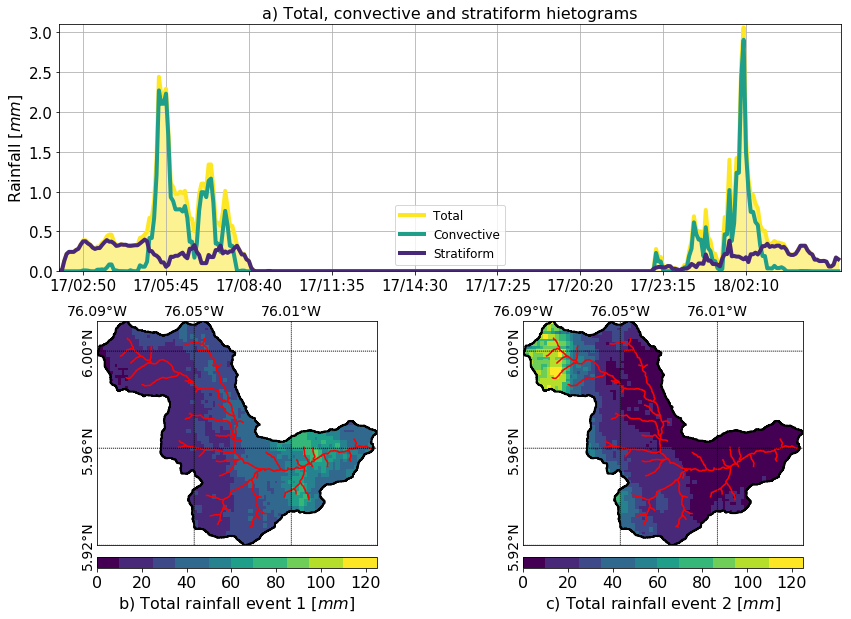
\includegraphics[width=8.3cm]{Figures/Rainfall_separation.png}
%DIFDELCMD <  %%%
%DIFDELCMD < \caption{%
{%DIFAUXCMD
\DIFdelFL{a) Temporal evolution of the convective-stratiform rainfall partitioning during both Events 1 and 2. The figure shows the total rainfall (yellow), and the convective (blue) and stratiform (green) portions integrated over La Liboriana basin. b) and c) Spatial distribution of the cumulative rainfall during Events 1 and 2 over La Liboriana basin.}}
    %DIFAUXCMD
%DIFDELCMD < \label{fig:separacionLluvia}
%DIFDELCMD < \end{figure}
%DIFDELCMD < %%%
\DIFdelend \DIFaddbegin \subsection{\DIFadd{Hydrologic model validation and sensitivity analysis}}
\DIFaddend 

Figure \ref{fig:SimStreamflow}a presents the results of the hydrological simulation at the outlet of the basin.  The model simulation is set to reach a base flow of 3 \DIFdelbegin \DIFdel{$m^3/s$}\DIFdelend \DIFaddbegin \DIFadd{m$^3 \text{s}^{-1}$}\DIFaddend , a value that corresponds to the discharge measurements during field campaigns days and weeks after the flash flood event and during dry spells.   The simulation shows that Event 1 generates a hydrograph with a peak flow of $Q_{max}$ = 160 \DIFdelbegin \DIFdel{$m^3/s$ that did not result in casualties or infrastructure losses, but }\DIFdelend \DIFaddbegin \DIFadd{m$^3 \text{s}^{-1}$. It is important to note that during precipitation Event 1 there were no damage nor flooding reports by local authorities. Even though this precipitation event did not generate  flooding, it }\DIFaddend set wet conditions in the entire basin before the occurrence of Event 2  (see the purple line in Figure \ref{fig:SimStreamflow}b). Additionally,  it is clear from the simulation that during the flash flood event the two successive convective cores over the same region (training convection) generated a peak flow of $Q_{max}$ =220 \DIFdelbegin \DIFdel{$m^3/s$}\DIFdelend \DIFaddbegin \DIFadd{m$^3 \text{s}^{-1}$}\DIFaddend , value that is in the upper range of the estimated streamflow based on \DIFdelbegin \DIFdel{a posteriori }\DIFdelend \DIFaddbegin \DIFadd{post-event }\DIFaddend field evidence (185-222 \DIFdelbegin \DIFdel{$m^3/s$}\DIFdelend \DIFaddbegin \DIFadd{m$^3 \text{s}^{-1}$}\DIFaddend ). Figure \ref{fig:SimStreamflow}a also presents the \DIFaddbegin \DIFadd{simulated }\DIFaddend runoff and subsurface flow separation as well as the convective-stratiform generated discharge discrimination.  The \DIFaddbegin \DIFadd{modeling }\DIFaddend evidence during Event 2 suggests the convective rainfall fraction dominates \DIFaddbegin \DIFadd{the }\DIFaddend hydrograph formation. In both events, convective (stratiform) precipitation appears to be closely related to \DIFaddbegin \DIFadd{the simulated }\DIFaddend runoff (subsurface flow).  On the other hand, \DIFaddbegin \DIFadd{the simulated }\DIFaddend subsurface flow is more important in magnitude than runoff \DIFaddbegin \DIFadd{in }\DIFaddend describing Event 1, while runoff is more relevant for Event 2. \DIFdelbegin %DIFDELCMD < \\
%DIFDELCMD < 

%DIFDELCMD < \begin{figure}[t]
%DIFDELCMD < \centering
%DIFDELCMD <  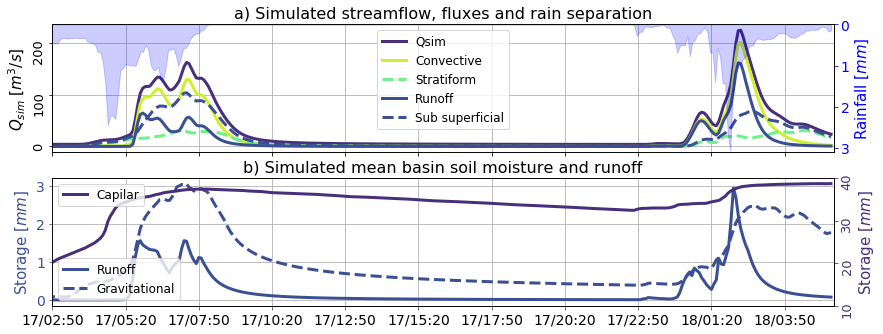
\includegraphics[width=12cm]{Figures/Caudal_Sim.png}
%DIFDELCMD <  %%%
%DIFDELCMD < \caption{%
{%DIFAUXCMD
\DIFdelFL{Summary of the Results from the hydrological simulation. a) Simulated streamflow,  runoff and sub-superficial flow separation and convective-stratiform generated discharge discrimination. b) Mean runoff, gravitational, and capillary storages during the simulation period.}}
    %DIFAUXCMD
%DIFDELCMD < \label{fig:SimStreamflow}
%DIFDELCMD < \end{figure}
%DIFDELCMD < 

%DIFDELCMD < %%%
\DIFdelend Figure \ref{fig:SimStreamflow}b presents capillary storage (purple), as well as runoff (continuous blue) and gravitational (dashed blue) storage temporal variability.  As expected, runoff storage is only non-zero during the storm duration, while gravitational storage increases considerably during rain events, followed by a slow recession.  There is an increment of basin-wide capillary storage during Event 1, remaining considerably high the time leading to the occurrence of Event 2. \DIFaddbegin \DIFadd{According to the model simulations, the peak flow occurred around 2:20 a.m. on May 18th, which is very accurate compared to the reports from local authorities considering all the data limitations.}\\

\begin{figure}[t]
\centering
 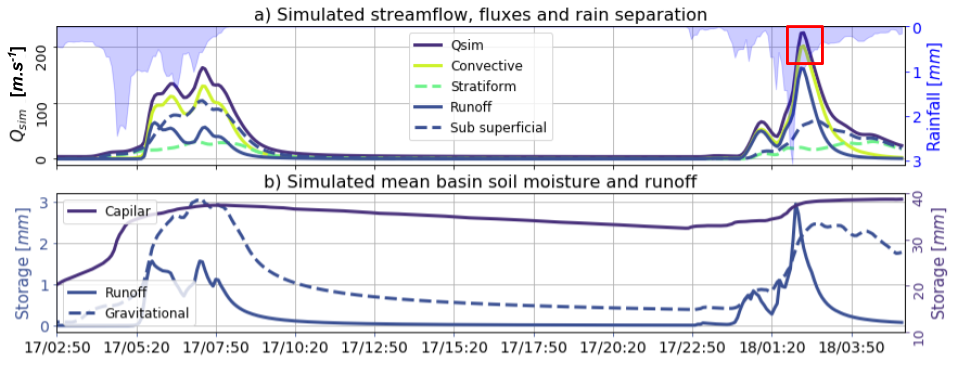
\includegraphics[width=12cm]{Figures/Caudal_Sim_v2.png}
 \caption{\DIFaddFL{Summary of the Results from the hydrological simulation. a) Simulated streamflow,  runoff and sub-surface flow separation and convective-stratiform generated discharge discrimination. The red square represents the flash flood peakflow interval estimated based on  field campaing evidence. b) Mean runoff, gravitational, and capillary storages during the simulation period.}}
    \label{fig:SimStreamflow}
\end{figure}

\DIFadd{Figure \ref{fig:SimStreamflowSA} shows the results of a sensitivity analysis of the hydrological simulation during the second rainfall event, varying the infiltration rate, and the surface and subsurface speed parameters. The aim of the sensitivity analysis is to evaluate the robustness of the overall results, considering the fact that the quality and quantity of some of the watershed information is limited. The overall simulation sensitivity results show the main findings  described in the previous paragraphs are, in fact, robust to almost all changes in the mentioned parameters, with surface runoff associated with convective rainfall controlling the magnitude of the peak discharge during the Event 2. Changes in the infiltration rate (Figure \ref{fig:SimStreamflowSA}a) result in peak flow changes with a magnitude less than 7\%,  and changes in the subsurface velocity parameter (Figure \ref{fig:SimStreamflowSA}c) lead to peak flow changes with a magnitude less than 20\% the original simulation. The model highest sensitivity, and hence the largest uncertainty source, appears to be related to the surface speed parameter (Figure \ref{fig:SimStreamflowSA}b), particularly in the low-end values. Although some of the surface speed values used in the analysis are unrealistically low,  it is noteworthy to report that these values lead to the attenuation of the hydrograph and the reduction of the peak flow. }\DIFaddend \\

\DIFaddbegin \begin{figure}[t]
\centering
 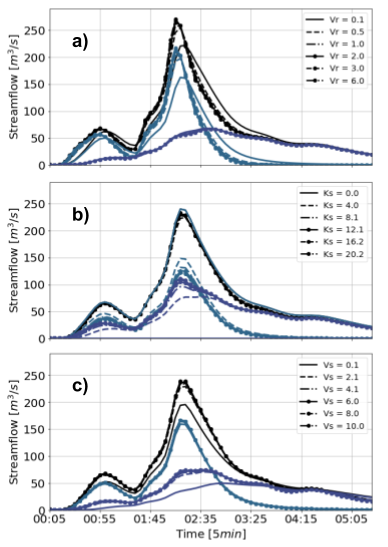
\includegraphics[width=14cm]{Figures/Parameter_variation_analysis.png}
 \caption{\DIFaddFL{Hydrological simulation sensitivity analysis. Similarly as in Figure \ref{fig:SimStreamflow}, all panels show the simulated streamflow, and the runoff and sub-surface flow separation. The left panel shows sensitivity to changes in the infiltration rate  parameter, the middle panel to changes in surface speed, and the right panel to changes in subsurface speed.}}
    \label{fig:SimStreamflowSA}
\end{figure}



\DIFadd{Figure \ref{fig:dischargeEvent2} shows the temporal evolution of discharge during Event 2 in different locations along the watershed's main channel. The upper location corresponds to 15\% of the area of the basin, and the other downstream locations to 52\%, 76\%, and 100\% of the watershed, respectively. In terms of volume, 73 Mm$^3$ of the total 144 Mm$^3$ simulated at the outlet of the basin are generated on the 15\% upstream part of the watershed,  corresponding to about half of the total mass. In terms of peak flow, due to the slope and velocity changes, the simulated discharge at the 15\% upstream part of the watershed corresponds to 61\% of the peak discharge at the outlet of the basin.}\\


\begin{figure}[t]
\centering
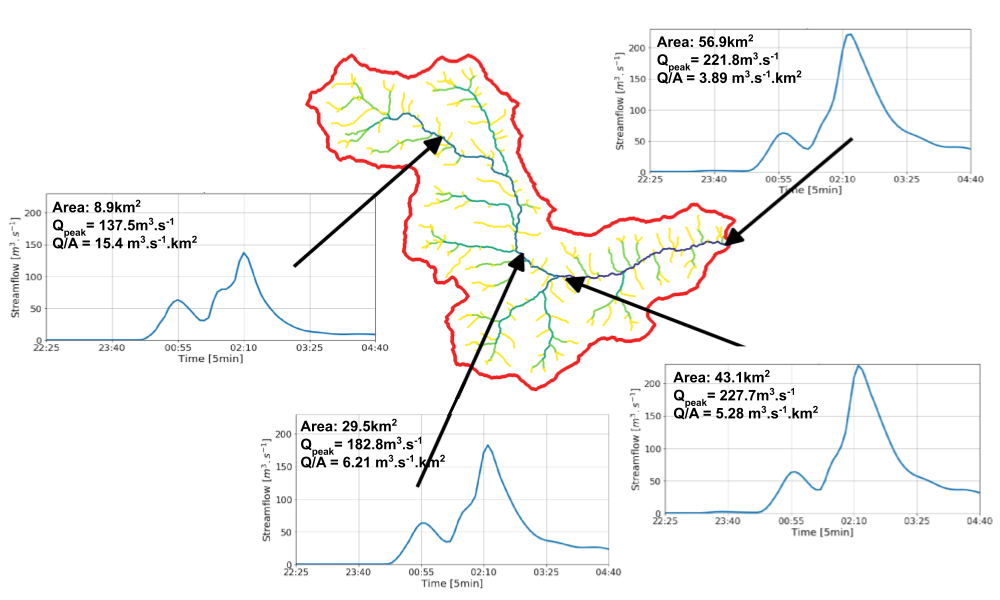
\includegraphics[width =12cm]{Figures/Evolucion_evento.png}
\caption{\DIFaddFL{Temporal evolution of discharge during Event 2 in different locations along the watershed's main channel. The upper location corresponds to 15\% of the area of the basin, and the other downstream locations to 52\%, 76\%, and 100\% of the watershed, respectively.}}
\label{fig:dischargeEvent2}
\end{figure}

\subsection{\DIFadd{Flash flood processes}}

\DIFaddend In this study, we propose a graphical method to assess the soil-rainfall-discharge coupling holistically. The first step is to classify all the cells within the watershed in a predetermined number of groups according to their localization and the distance to the outlet. The aim is to establish a coherent and robust spatial discretization, thus allowing to summarize the concurrent spatio-temporal variability of the different processes in 2D diagrams.\DIFdelbegin \DIFdel{Figure \ref{fig:ExplainationGroups} presents an example of the spatial structure of cell grouping for La Liboriana basin using 10 (left) and 50 (right) groups.}\DIFdelend \\

\DIFdelbegin %DIFDELCMD < \begin{figure}[t]
%DIFDELCMD < \centering
%DIFDELCMD <  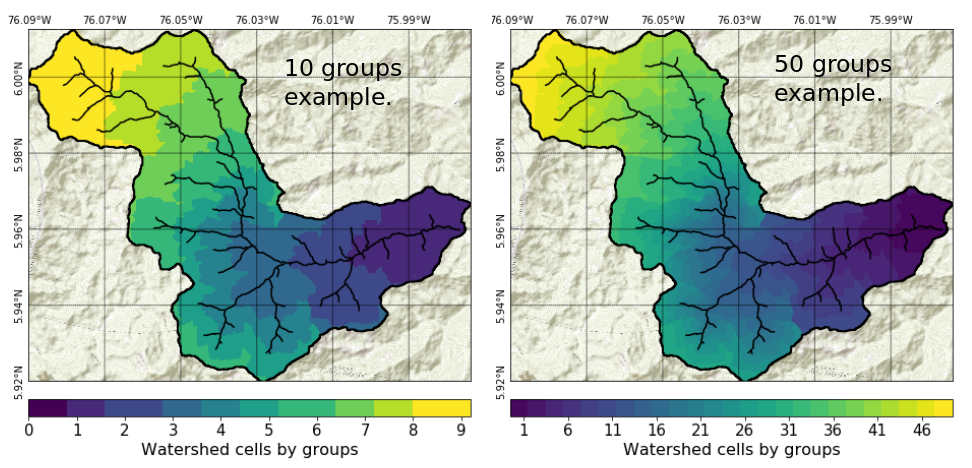
\includegraphics[width=8.3cm]{Figures/Mapas_Grupos.png}
%DIFDELCMD <  %%%
%DIFDELCMD < \caption{%
{%DIFAUXCMD
\DIFdelFL{Example of watershed grouping as a function of distance to the outlet for La Liboriana basin. The left panel corresponds to clustering using ten different groups, and the right panel shows the 50-groups categorization used in the present study.}}
    %DIFAUXCMD
%DIFDELCMD < \label{fig:ExplainationGroups}
%DIFDELCMD < \end{figure}
%DIFDELCMD < %%%
\DIFdelend %DIF >  \begin{figure}[t]
%DIF >  \centering
%DIF >  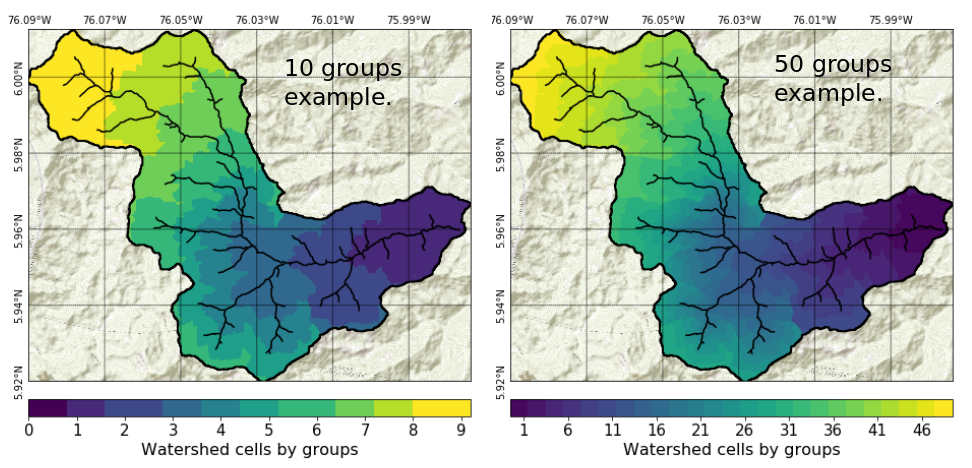
\includegraphics[width=8.3cm]{Figures/Mapas_Grupos.png}
%DIF >  \caption{Example of watershed grouping as a function of distance to the outlet for La Liboriana basin. The left panel corresponds to clustering using ten different groups, and the right panel shows the 50-groups categorization used in the present study.}
%DIF >  \label{fig:ExplainationGroups}
%DIF >  \end{figure}

Figure \ref{fig:HumedadSpatioTemporal} presents the proposed 2D diagrams obtained for the simulation of the La Liboriana basin flash flood using a spatial discretization with 50 groups. Figure \ref{fig:HumedadSpatioTemporal}a includes the evolution of the average rainfall over the basin (black line), and the spatio-temporal evolution of capillary storage (filled isolines) and return flow (colored isolines from white to red) by groups. For the analysis, it is relevant to highlight that higher numbered groups are located away from the outlet of the basin and correspond in this case to considerably steeper slopes. Figure \ref{fig:HumedadSpatioTemporal}b presents the evolution of streamflow at the outlet of the basin (black line) as well as the gravitational storage (filled isolines) and runoff (colored isolines) spatio-temporal evolution.  \DIFaddbegin \DIFadd{Figure \ref{fig:HumedadSpatioTemporal} shows  variations in the capillary and gravitational storages associated with Event 1 in the higher numbered groups.  The capillary storage remains high in almost all the basin until the start of Event 2.  According to the conceptualization of the model, the gravitational storage and surface runoff start to interact when the capillary storage is full. In this case, this situation is set up by Event 1.  Model runs for Event 2 using dry initial states, show no flooding in the results.}\DIFaddend \\

\begin{figure}[t!]
\centering
 \DIFdelbeginFL %DIFDELCMD < 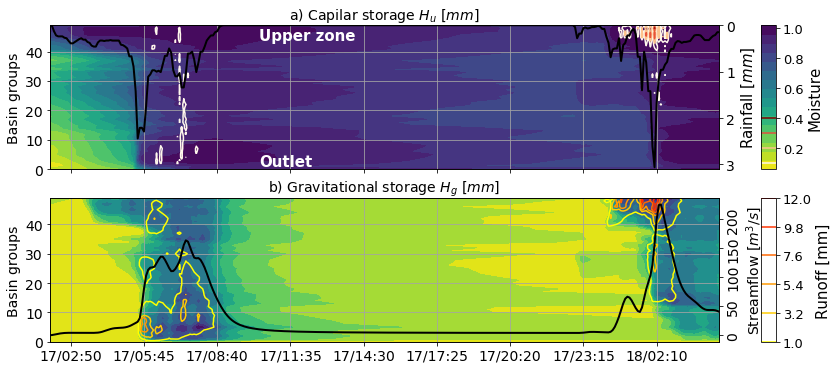
\includegraphics[width=12cm]{Figures/Evolucion_humedad.png}
%DIFDELCMD <  %%%
\DIFdelendFL \DIFaddbeginFL 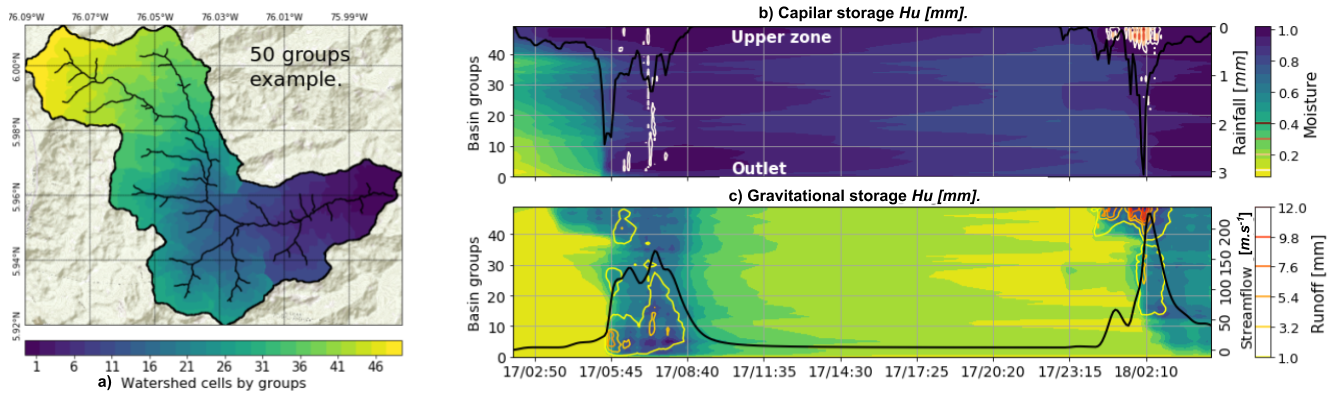
\includegraphics[width=12cm]{Figures/Figure_9_10.png}
 \DIFaddendFL \caption{\DIFdelbeginFL \DIFdelFL{Spatiotemporal }\DIFdelendFL \DIFaddbeginFL \DIFaddFL{Watershed groups and spatiotemporal }\DIFaddendFL analysis of Events 1 and 2.  a) \DIFaddbeginFL \DIFaddFL{Example of watershed grouping as a function of of their localization and distance to the outlet for La Liboriana basin using a 50-groups categorization. Each group corresponds to a row in the contour plots b) and c). b) }\DIFaddendFL Simulated capillary moisture (filled green-to-blue contours) and returned flow occurrence (white to red isolines).  The black line represents the average rainfall over the basin. \DIFdelbeginFL \DIFdelFL{b}\DIFdelendFL \DIFaddbeginFL \DIFaddFL{c}\DIFaddendFL ) Simulated gravitational moisture (filled green-to-blue contours) and runoff (yellow-to-red isolines).  The black line represents streamflow at the outlet of the basin.  The green-to-blue color bar serves as a reference for capillary moisture and gravitational water content.}
    \label{fig:HumedadSpatioTemporal}
\end{figure}

It is well known that \DIFaddbegin \DIFadd{the }\DIFaddend temporal variability of rainfall intensity plays an important role in \DIFaddbegin \DIFadd{the  }\DIFaddend hydrograph structure. During Event 1 rainfall accumulated over the basin at a relatively stable rate (Figure \ref{fig:lluviaElapsedCaudal}a).  On the other hand, Event 2 presents a significant increase in rainfall rate in the second half of the life cycle (Figure \ref{fig:lluviaElapsedCaudal}b).  This change in precipitation intensity is associated with a considerable intensification of the training convective cores due to orographic effects. Events 1 and 2 also exhibit differences in the elapsed time between rainfall occurrence and streamflow increment given the relative timing of stratiform versus convective rainfall (see the gray band in Figure \ref{fig:lluviaElapsedCaudal}a and b).  For Event 1, the median elapsed time between rainfall and streamflow ($Et_{p50}$) is 1.12 hours while for Event 2 $Et_{p50}$ is 0.79 hours.  The median elapsed time between the convective portion and the streamflow ($Etc_{p50}$) in Event 1 is 0.75 and 0.46 in Event 2. The minimum value of the convective elapsed time $Etc_{min}$ also descends from 0.42 to 0.25 hours.  On the other hand, there is an increase of median elapsed time between stratiform rainfall and streamflow ($Ets_{p50}$) from 1.21 to 1.83 hours.  In Event 2, the convective rainfall and the runoff show a similar evolution,  denoting a strong influence of the convective portion (Figure \ref{fig:lluviaElapsedCaudal}b).\\

\begin{figure}[t]
\centering
 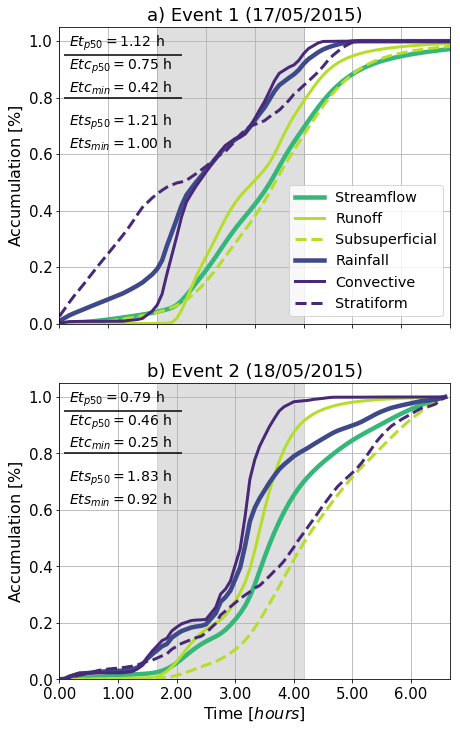
\includegraphics[width=8.3cm]{Figures/Rain_Streamflow_Elapsed.png}
 \caption{Accumulated rainfall and streamflow for a)  Event 1 and b) Event 2. The accumulation is expressed in percentage respect to the total value in each case. Median elapsed time and minimum elapsed time () are estimated between total ($Et_{p50}$, $Et_{min}$), convective ($Etc_{p50}$, $Etc_{min}$), and stratiform ($Ets_{p50}$, $Ets_{min}$) rainfall and the runoff portion of the streamflow.  Gray bands correspond to the periods for elapsed time estimation.}
    \label{fig:lluviaElapsedCaudal}
\end{figure}

As mentioned before, average rainfall accumulation over the basin for Events 1 and 2 is 47$mm$ and 38$mm$, respectively. During  Event 1 (2), convective (stratiform) average accumulations are 28 (23) and 17 (14) $mm$, respectively (Figure \ref{fig:RainAcumByReach}a and b).  The maximum rainfall intensities are relatively similar with 150$mm/h$ and 180$mm/h$ for Events 1 and 2, respectively.  Despite this, Event 1 does not trigger a flash flood event. The overall evidence suggests that the discriminating factor between both events does not lie in the portions of convective or stratiform rainfall but rather in their spatial distribution. \\

Figures \ref{fig:RainAcumByReach}a and b, and Figures \ref{fig:RainAcumByReach}c and d show the convective and stratiform cumulative rainfall, and the spatially-averaged convective and stratiform rainfall, both as a function of sub-basin reach, respectively.  Figures \ref{fig:RainAcumByReach}a and b show that while  Event 1 exhibit similar convective and stratiform rainfall accumulation for different watershed scales, Event 2 shows a more significant cumulative contribution of convective rainfall than of stratiform precipitation. Convective rainfall tends to cover less area, and at the same time present a spatio-temporal erratic behavior \citep{Steiner1995, Houze1989}. Figures \ref{fig:RainAcumByReach}c and d provide evidence that convective rainfall present higher variations at small sub-basins than for a larger-order basin. During Event 2, convective accumulation reaches higher values for small and medium sub-basins.   Convective rainfall occurrence at the upper sub-basins has significant implications due to geomorphological conditions associated to zero-order sub-basins \citep{Sidle2018}. Figure \ref{fig:PearsonCorr} presents Pearson correlations coefficients between the convective and stratiform hydrograph portions and the runoff and subsurface flow. According to this, convective and stratiform rainfall exhibit a weaker relationship with the flow characteristics at small scales (under 5$km^2$).  This is likely to be associated with increasing variability of rainfall and hydrograph formation at small scales \citep{Ayalew2014}.  Correlations tend to grow with increasing  area, indicating stabilization of the hydrograph formation. Additionally,  subsurface flow presents higher correlations during Event 1, while correlations with runoff are higher for Event 2, highlighting the most important process in each case.  The relevance of subsurface flow is likely due to the rainfall characteristics during  Event 1, with homogeneous rainfall intensity and high rate of basin recharge (see Figure \ref{fig:SimStreamflow}b).  On the other hand, saturation processes and a wet soil profile explain the observed higher correlations during Event 2. \\

\begin{figure}[t]
\centering
 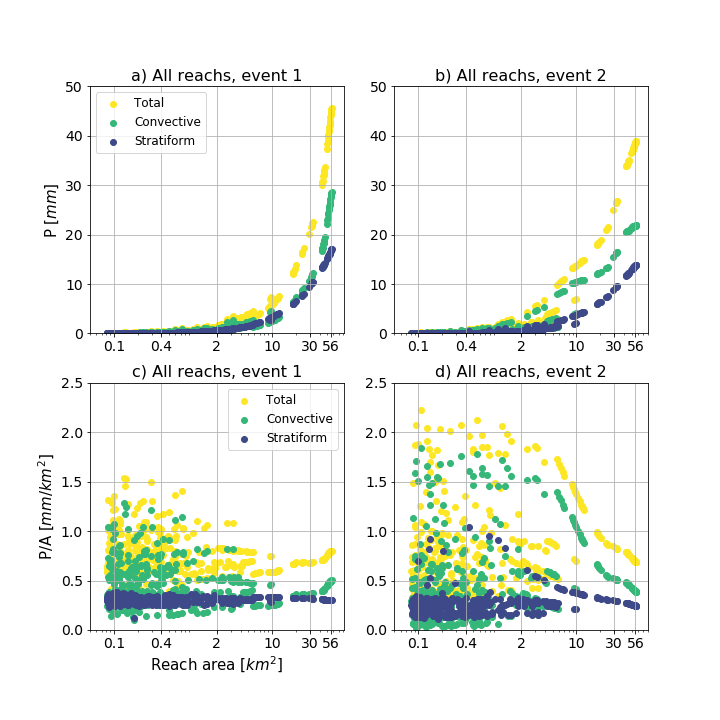
\includegraphics[width=8.3cm]{Figures/RainAcum_by_reach.png}
 \caption{Cumulative rainfall versus the area at each reach of the basin for a) Event 1 and b) 2. Panels c) and d) show the average rainfall versus the area at each reach of the basin. Yellow dots correspond to the total, green dots to convective and blue dots to stratiform rainfall. All panels use a logarithmic scale for the basin area.}
    \label{fig:RainAcumByReach}
\end{figure}

\begin{figure}[t]
\centering
 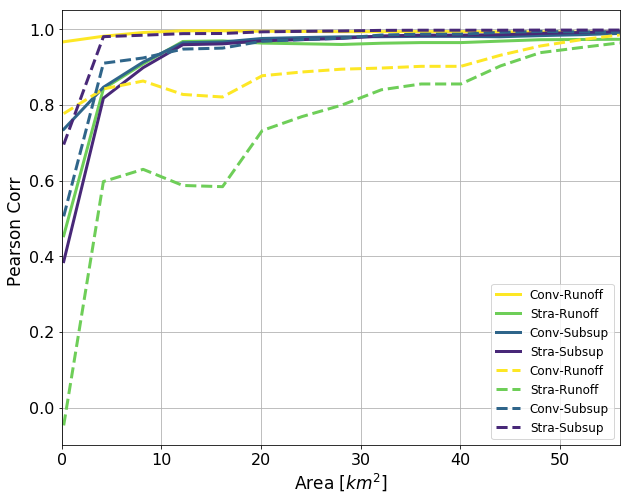
\includegraphics[width=8.3cm]{Figures/CorrPearson_TipoRain_Fluxes.png}
 \caption{Pearson correlations among convective and stratiform portions of the rainfall and runoff and subsurface flow for different reach areas. Dashed lines correspond to Event 1 and continuous lines Event 2.}
    \label{fig:PearsonCorr}
\end{figure}


\subsection{Landslide and \DIFdelbegin \DIFdel{Flood Simulations}\DIFdelend \DIFaddbegin \DIFadd{flood simulations}\DIFaddend }

In addition to the hydrological simulation, associated hazards such as floods and landslides are also modeled and discussed in this study. The landslides model as described in the previous section requires additional information including soil depth $Z$, cohesion $C'$, friction angle $\phi$ and specific weight $\gamma$.  According to the  description by  \citet{Osorio2008}, illustrating a clay-slime soil,   $C'$  is  assumed equal to 4$KN$, $\phi$ to 30$^0$ and $\gamma$ to 18; $Z$ vary with slope according to Table \ref{tab:suelos}. \\

Figure \ref{fig:SlidesComparison}a presents the observed landslides triggered by Event 2  based on aerial photos and satellite images (Landsat/Copernicus, and Google) taken before and after the flash flood.  Figure \ref{fig:SlidesComparison}b shows,  by hills, the map of total unstable cells during the simulation period, and Figure \ref{fig:SlidesComparison}c shows the time series of the number of simulated unstable cells during Event 2 (continuous purple line) and the mean rainfall over the basin (inverse axes, blue line). Calibration of the landslide model was performed by finding the maximum overlap between simulated and observed unstable and stable cells, and at the same time reducing the overall number of false positives and false negatives. It is important to note that the calibration strategy is not a cell-by-cell modification of the parameters involved but rather a basin-wide modification of soil properties. A sensitivity analysis of soil parameters is carried out by making small variations of the variables within specified intervals: $\phi$ between 25 and 32, $\gamma$ between 17 and 19,  $C'$ between 3.5 and 4.2, and $Z$ between 0.1 and 3 $m$ . The sensitivity analysis suggests that slight variations in the parameter in $Z$ produce significant changes in the modeled landslides, resulting in an overestimation of the number of unstable cells, or no unstable cells at all. Following Table \ref{tab:suelos}, the average soil depth in the basin is only 0.3 m, a value that corresponds to underestimation according to the inspections during field visits. For this reason, the results presented in Figure \ref{fig:SlidesComparison} use a  $Z$ map scaled by a calibration factor of 3.5, preserving the spatial dependence on the slope, but achieving a more realistic soil depth and better spatial distribution of landslide occurrence.\\ 


\begin{figure}[t!]
\centering
 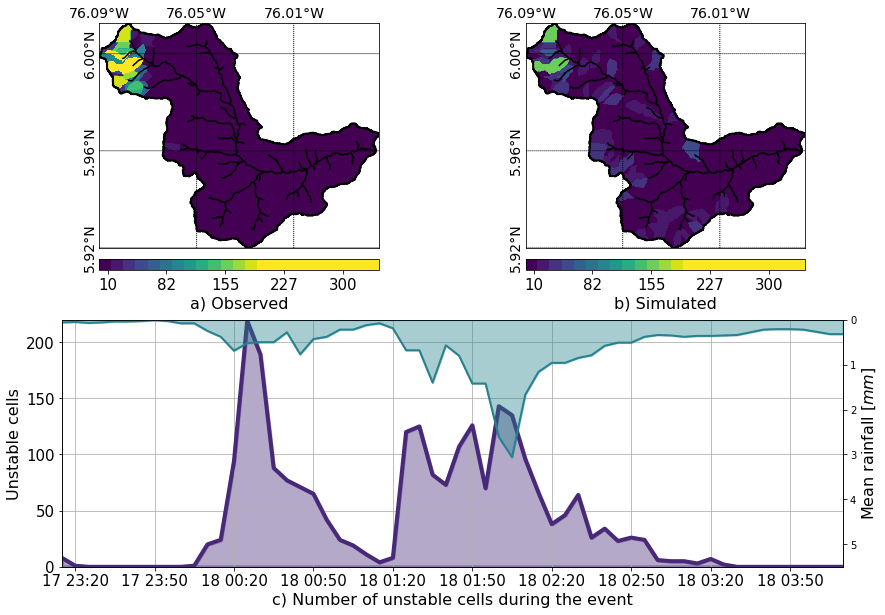
\includegraphics[width=12cm]{Figures/Slides_byHills.png}
 \caption{a)  Observed landslides triggered by Events 1 and 2. The figure is based on aerial photos and satellite images (Landsat/Copernicus, and images available on Google) taken before and after the flash flood event.  b) Map of total unstable cells during the simulation period. c) Time series of number of simulated unstable cells during Event 2 (continuous purple line) and mean rainfall over the basin (inverse axes, blue line).}
    \label{fig:SlidesComparison}
\end{figure}

The model represents considerably well the spatial distribution of the areas that are prone to trigger shallow landslides during Event 2, showing a significant density of unstable cells in the hills where slides took place. However, despite the calibration efforts, the total number of unstable cells is relatively low compared to observations. \DIFaddbegin \DIFadd{It is important to note that there was no spatial calibration in order to obtain the right location of the landslides. The calibration only includes the change of the soil depth using a single scalar, constant for the entire basin, in order to maximize the number matching observed and simulated slides. In other words, there is just one single basin-wide parameter modified, and not an independent modification of the parameter for every pixel in order to obtain the right distribution.  This is important because in that sense, it serves to check the capability of the model to estimate risk areas only considering  topography and rainfall data. }\DIFaddend A pinpoint localization of the unstable cells is still considered a hard task in part due to the small temporal and spatial scale at which landslide processes take place \citep{Aristizabal2016, Dhakal2004, Wu1995}. Additionally,  the lack of detailed soil information increases the simulation uncertainty. Notwithstanding the difficulties, the results suggest that the model simulations could have been used and should be used in the future for early detection and warning to improve both short and long-term risk reduction strategies.\\


\DIFdelbegin \DIFdel{According to the model results, a significant portion of the landslides happened during the first of the training convective cores reaching the upper basin (see Figure \ref{fig:SlidesComparison}c).  Due to the high soil moisture, cells located in the mentioned region where prone to failure. The second and more intense convective core, between 1:20 and 2:15 a.m.,  also triggered additional slides for an extended period.  During storm events, shallow landslides become a significant source of gravels and sediments.  These particles tend to reach the river network, increasing the magnitude of the streamflow and its destructive power.  Despite this, there is no current explicit link in the model between the landslides scheme and the hydraulic submodel.  Nonetheless, HydroFlash assumes that sediment transport is limited by channel capacity, and not by hillslope supply, which in this case is guaranteed by the elevated number of landslides.}%DIFDELCMD < \\  
%DIFDELCMD < 

%DIFDELCMD < %%%
\DIFdelend Figure \ref{fig:SimFloodSpots} shows the identification of the flood spots at the peak of Event 2 (May 18th, 2015, 2:00 a.m.) as simulated using HydroFlah. Figures \ref{fig:SimFloodSpots}b to f present a detail view of the results from the outlet of the basin to the upper region.  Cases presented in Figures \ref{fig:SimFloodSpots}e and f exhibit a satisfactory agreement with observed flood spots (blue shadow).  Cases in Figures \ref{fig:SimFloodSpots}c and d also show a good approximation, but with minor spatial shifts in some sections. The largest spatial differences are observed in Figures \ref{fig:SimFloodSpots}b. At the entrance of the urban zone, the model overestimates the flood spots.  The model results indicate that 11\% of flood spots happen at elements of order 1 and 2,  and, 18, 38 and 32\% happen at orders 3, 4 and 5, respectively.  This also highlights a coherent geomorphological representation of the flooded channels and hills with the order.\\   

\begin{figure}[t!]
\centering
 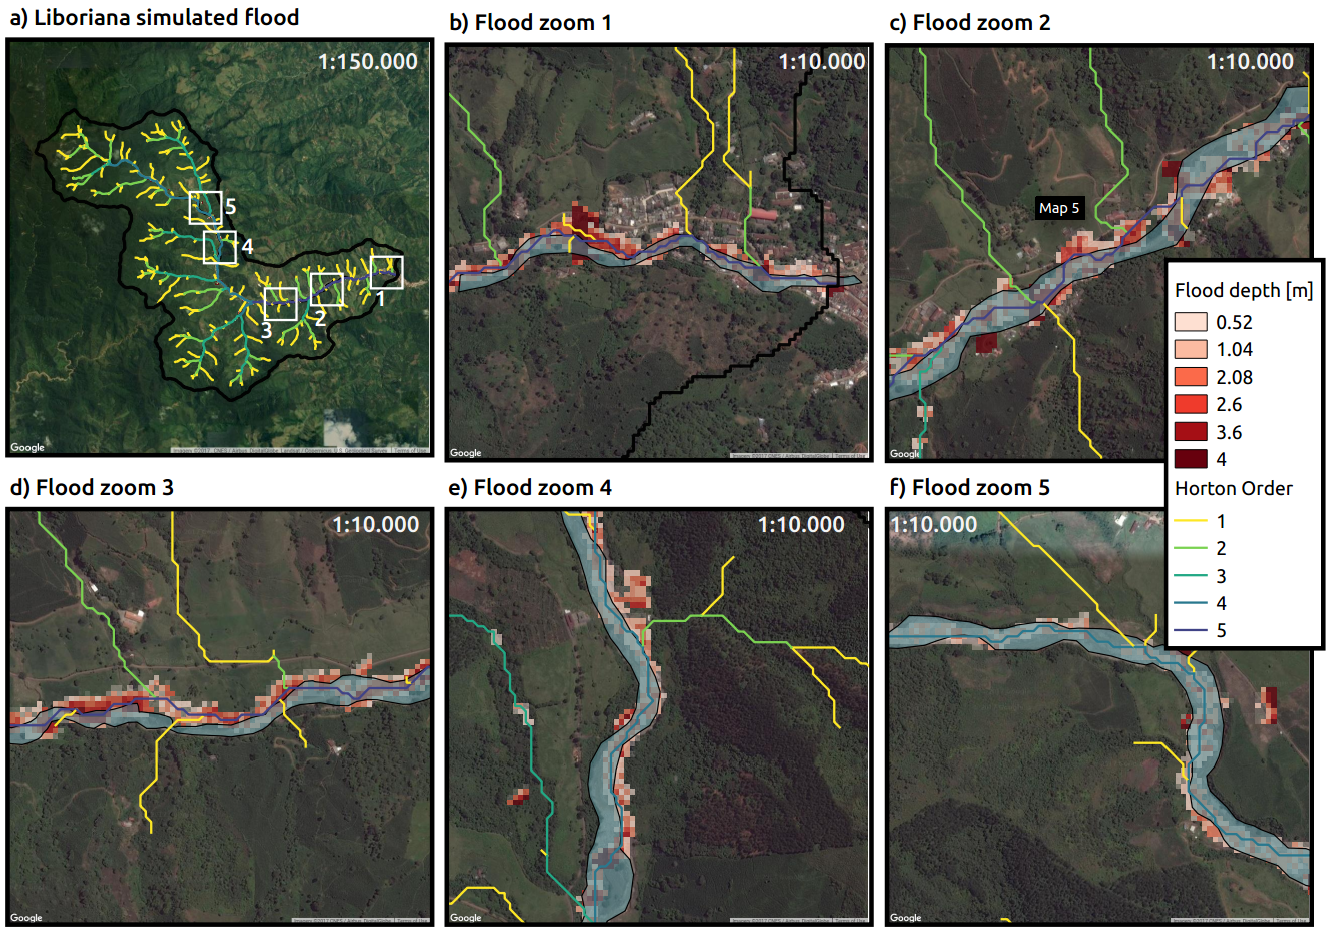
\includegraphics[width=12cm]{Figures/Manchas2.png}
 \caption{Simulated flood spot at the peak of Event 2 in different locations. a) Basin drainage network. White squares correspond to regions of interest highlighted in panes b) to f). \DIFaddbeginFL \DIFaddFL{The colors of the streams correspond to the Strahler order of the network. }\DIFaddendFL b) Zoom at the outlet of the basin, where an important portion of the human and infrastructure loses took place. c) Zoom at La Margarita settlement also affected by the flash flood. d) to f) Zoom at key locations along the principal stream.  Observed flood spots are shown in blue polygons and model flood spots in red to white grids.}
    \label{fig:SimFloodSpots}
\end{figure}

\DIFdelbegin %DIFDELCMD < \vspace{5cm}
%DIFDELCMD < %%%
\DIFdelend %DIF > \vspace{5cm}
%%-----------------------------------------------------------
%%-----------------------------------------------------------
%Discussion
%%-----------------------------------------------------------
%%-----------------------------------------------------------

\section{Discussion}
\label{sec:discussion}

During the morning of May 18th of 2015,  \DIFdelbegin \DIFdel{1:30 a.m local time,  }\DIFdelend a flash flood occurred in the steep La Liboriana basin, in the municipality of Salgar,  Department of Antioquia, Colombia, leaving more than 100 human casualties, 535 houses destroyed, and significant infrastructure loses.  \DIFdelbegin \DIFdel{The disaster was reported to departmental and national authorities around 2:00 and 2:30 a.m. }\DIFdelend Due to the lack of local information of soil type, land use and real-time hydrometeorological data, La Liboriana case implies a challenge for flash flood prediction, modeling and, consequently, risk management.  The present paper introduces a \DIFdelbegin \DIFdel{hydrological }\DIFdelend \DIFaddbegin \DIFadd{hydrologic }\DIFaddend model-based approach and an integral graphical analysis tool (an integrated spatiotemporal analysis of rainfall evolution, together with soil storages in the basin),  not only to simulate and understand all the relevant soil-rainfall-discharge processes that  led to the 2015 Salgar flash flood while assessing the associated natural hazards, but also to propose it as a radar QPE-based landslide and flash flood guidance low-cost tool for basins with scarce data and regions with limited resources. \\

The methodology implies the development of a distributed \DIFdelbegin \DIFdel{hydrological }\DIFdelend \DIFaddbegin \DIFadd{hydrologic }\DIFaddend model with the capabilities of tracking independently convective and stratiform precipitation within the model as well as keeping track of the runoff and subsurface portions of the streamflow,  coupling a shallow landslide submodel and a one-dimensional flash flood scheme (HydroFlash).  The model proposed here indeed allows studying the different hydrological processes relevant to flash flood and landslide occurrence by using different simulation resources, serving as the basis for a better understanding of the overall basin response. This overall approach helps to isolate flood generating mechanisms or causative factors both in time and also in space, focusing on the important physical processes and not only on \DIFdelbegin \DIFdel{the }\DIFdelend statistics \citep{klemes1993, Merz2003}. It is hoped that knowledge improvement leads to the anticipation of the warning and response by risk management entities. \\

The evolution of the simulation of Events 1 and 2 show evidence of remarkable behavioral differences. During Event 1 both gravitational and capillary tanks are filled along and across the basin as a result of the quasi-homogeneous rainfall spatial distribution. The return flow is low, and most of the runoff occurs within the first 20 groups (40\% of the watershed closest to the outlet).   In the period between both events, there is a recession in the capillary and gravitational storages in the entire basin. Capillary storage decays considerably slower than gravitational storage.  During Event 2, the flash flood \DIFaddbegin \DIFadd{triggering }\DIFaddend event,  the first convective core saturates both capillary and gravitational storages in the upper part of the basin and generates both return flow and significant runoff.   Due to soil saturation, the second convective core results mainly in surface runoff. During this event, runoff is generated the lower part of the basin while extreme runoff rates are evident in the upper part of the basin, collocated with the steeper slopes. On the other hand, subsurface flow is more important in magnitude than runoff describing Event 1, while runoff is more relevant for Event 2. The precedent storage and the presence of thunderstorm training profoundly condition the streamflow during Event 2. The overall evidence suggests that precedent capillary moisture in the basin plays an essential role in modulating river discharge. This behavior could be linked to the temporal occurrence and relative importance and timing of stratiform and convective formations previously described. \\

While convective and stratiform partitioning could influence the runoff and subsurface flow separation,  the spatial distribution of rainfall relative to watershed network morphometry structure impose a condition on the hydrological response of the basin. In other words, hydrograph formation is not only determined by the rainfall accumulation or maximum intensity, but also by its spatial structure. The structure of the rainfall associated with La Liboriana event highlights the need to consider in more detail the role of orographic rainfall intensification in practical applications such as early warning systems. Evidence suggests the spatial structure of the rainfall is at least as important as the geomorphological features of the basin regulating the generation of flash flood events.\\

An integrated spatiotemporal analysis of rainfall evolution, together with soil storages in the basin is necessary to study the relevance of antecedent conditions and precipitation type, intensity, and location in the generation of flash flood events.  Event 1 increased the overall soil moisture with an associated decrease on infiltration rates similar to results reported by \citet{Penna2011} and \citet{Zehe2010}, low infiltration increase runoff rates, which finally affects the susceptibility of the basin to  flash floods occurrence \citep{Wagner1999,Penna2011,Tramblay2012b}. La Liboriana geomorphological characteristics, corresponding to a steep tropical basin, determine the potential energy that controls water transit velocity.  Water tends to reach faster the channels in order 1 and 2 hills, and, at the same time, the sediment production and transport in these hills tend to be larger.  Order 3 sub-basins most likely act as transport elements, with no important energy losses. Floods tend to occur in order 4 and 5 sub-basins due to the widening of the channel and slope attenuation. \\

Different authors have focused on trying to understand the general causative factors behind the occurrence of flash floods finding similar to our results, a significant role of basing geomorphology, orography and local convection. For example, \citet{Lehmann2012}, using a shallow landslide model, finds an important role of the topography and the rainfall conditions.  \citet{Turkington2014} shows how intense locally driven convection appears to be the main meteorological trigger for flash occurrence in the French Alpes.\citet{Camarasa2016} shows how rainfall intensity and duration influences the shape of the hydrograph, with intense rainfall shortening the response time of the basin, and large durations increasing the flood peak. In the Mediterranean region, \citet{Boudou2016}  states that in addition to the rainfall, geomorphological characteristics and antecedent soil conditions are key in the generation of flash flooding.\\

However useful, the evidence in this work only takes into account two successive events; an analysis of more cases and different spatial scales (different basins) would provide robust conclusions in this direction. It is clear that it is not conclusive enough to focus on a single extreme event, rather than on a spectrum of floods \cite{Merz2003}.  The \DIFaddbegin \DIFadd{model simulation }\DIFaddend results suggest it is imperative to study in depth the long-term link between the relative basin and drainage network orientation and the preferred path of precipitation events and its role in defining the frequency of flash flood occurrence. A better understanding of the network-hills-preferential rainfall advection structure could provide information about basins prone to flash floods when information is scarce.\\


\conclusions[Conclusions]
\label{sec:conclusions}

Extreme rainfall events such as the one that triggered La Liboriana tragedy frequently take place in Colombia and the entire global tropical belt over ungauged basins, often triggering flash floods and torrential flows, endangering vulnerable communities due to poor long-term planning and lack of functional early warning systems. There is a global need for better knowledge and understanding of the hydrological and meteorological conditions that, combined, lead to the manifestation of natural hazards. Such understanding must result in useful practical applications that improve risk management practices saving lives. \DIFaddbegin \DIFadd{In the current work, we approach the problem from a hydrological modeling point of view, trying, despite the data limitations and the uncertainty of the results, to shed some light in the first-order processes that modulate the occurrence of flash floods in the region.  }\DIFaddend \\  

In the case of La Liboriana flash flood, radar reflectivity fields were available from a C-Band radar operated by the Early Warning System of Medellín and its metropolitan area as part of a local risk management strategy. While the municipality of Salgar is located far outside Medellín's metropolitan area, the radar is about \DIFdelbegin \DIFdel{60 }\DIFdelend \DIFaddbegin \DIFadd{90 }\DIFaddend km away from Salgar, and the reflectivity retrievals enable the classification of precipitation fields into convective and stratiform areas using widely accepted methodologies by the meteorological community.  Radar reflectivity is also a proxy for precipitation allowing a quantitative estimation \DIFaddbegin \DIFadd{of rainfall fields}\DIFaddend . This estimation was used together with the \DIFdelbegin \DIFdel{hydrological modeling }\DIFdelend \DIFaddbegin \DIFadd{hydrologic model }\DIFaddend to assess the different basin-wide processes taking place during the flash flood triggering rainfall event.  \DIFaddbegin \DIFadd{The limitations of the methodology presented in this work do not allow to represent all the detailed small-scale preferential pathways of water in the watershed, but rather focus on the first-order approximation to study the partitioning between runoff vs. subsurface flow. Also, the model results are used to obtain a conceptual idea about the general processes, but it must be taken into account that the simulations are subject to a calibration process that could lead to erroneous conclusions about the physical processes. This could be true even as different steps were taken trying to avoid this situation.  }\DIFaddend \\

The overall \DIFaddbegin \DIFadd{model simulation }\DIFaddend methodology reproduces considerably well the magnitude and timing of La Liboriana flash flood discharge peak, \DIFdelbegin \DIFdel{as well as }\DIFdelend \DIFaddbegin \DIFadd{showing robustness to changes in the most important model parameters, and reasonably well }\DIFaddend the areas of regional land-slide occurrence and flood spots location.  \DIFdelbegin \DIFdel{Simulation }\DIFdelend \DIFaddbegin \DIFadd{Model simulation }\DIFaddend results indicate that the flash-flood and the regional land-slide features were strongly influenced by the \DIFaddbegin \DIFadd{observed }\DIFaddend antecedent rainfall associated with a northeasterly stratiform event that recharged the gravitational and capillary storages \DIFaddbegin \DIFadd{in the entire basin}\DIFaddend . The hydrologic simulation shows that the antecedent event set wet conditions in the entire basin before the occurrence of the flash flood event, governing the streamflow during the latter.  \DIFdelbegin \DIFdel{The }\DIFdelend \DIFaddbegin \DIFadd{Results of the model simulation also suggest that the }\DIFaddend first of the two successive convective cores (thunderstorm training) over the same region during the \DIFaddbegin \DIFadd{second precipitation event (the }\DIFaddend flash flood event\DIFaddbegin \DIFadd{) }\DIFaddend saturated both capillary and gravitational storages in the upper part of the basin and generated both return flow and significant runoff.  The second convective core resulted mainly in surface runoff spatially collocated with the steeper slopes, generating the kinetic energy needed to produce La Liboriana flash flood. Overall results also show \DIFdelbegin \DIFdel{an excellent }\DIFdelend \DIFaddbegin \DIFadd{a good }\DIFaddend agreement between the simulated flood spots and the observed ones; this in spite of the limitations imposed by the resolution of the DEM used for extracting cross sections, and the model \DIFdelbegin \DIFdel{simplifications described in the Methodology section}\DIFdelend \DIFaddbegin \DIFadd{oversimplifications}\DIFaddend . \\

\DIFdelbegin \DIFdel{The }\DIFdelend \DIFaddbegin \DIFadd{Considering all the shortcomings and generalizations, the }\DIFaddend described model-based approach is \DIFdelbegin \DIFdel{useful to isolate }\DIFdelend \DIFaddbegin \DIFadd{potentially useful to assess }\DIFaddend flood generating mechanisms and as a tool for policy-makers\DIFaddbegin \DIFadd{, }\DIFaddend not only for short-term decisions in the context of an early warning system but also as a planning resource for long-term risk management. While several improvements \DIFdelbegin \DIFdel{could }\DIFdelend \DIFaddbegin \DIFadd{need to }\DIFaddend be implemented, including a better representation of hydraulic parameters,  and a \DIFaddbegin \DIFadd{direct }\DIFaddend link between landslides and flood spots similar to the strategy \DIFaddbegin \DIFadd{presented }\DIFaddend in the STEP-TRAMM model \citep{Fan2017a}, the results suggest it is possible to use  \DIFdelbegin \DIFdel{the }\DIFdelend low-cost \DIFdelbegin \DIFdel{methodology introduced here to not only improve our understanding of hydrological processes but also }\DIFdelend \DIFaddbegin \DIFadd{methodologies such as the one introduced here }\DIFaddend as a risk management tool in countries and regions with scarce resources.\DIFdelbegin \DIFdel{In the case of Salgar, there was radar information available, but in many cases, the only near-real-time precipitation information comes from satellite retrievals.  It would be very useful from a practical point of view to assess in which cases satellite information is enough for risk management applications. Comparing the Salgar case with the Mocoa (Department of Putumayo, Colombia)  April 1st, 2017 flash flood that resulted in more than 330 fatalities could help address this question.}\DIFdelend \\

% \appendix
% \section{}    %% Appendix A

% \subsection{}                               %% Appendix A1, A2, etc.

\section{Acknowledgements}
This work was supported by SIATA (Sistema de Alerta Temprana de Medellín y el Valle de Aburrá)  funds provided by Area Metropolitana \DIFdelbegin \DIFdel{de Medellín y }\DIFdelend del Valle de Aburrá (AMVA), Municipio de Medellín, Grupo EPM, and ISAGEN under the Research and Technology Contract CD511\DIFdelbegin \DIFdel{of }\DIFdelend \DIFaddbegin \DIFadd{, }\DIFaddend 2017.  \DIFdelbegin \DIFdel{Nicolás Velásquez was partly funded by }\DIFdelend Universidad Nacional de Colombia \DIFaddbegin \DIFadd{partly funded Nicolás Velásquez }\DIFaddend under the Facultad de Minas graduate scholarship program. \DIFaddbegin \DIFadd{Both authors would like to thank anonymous reviewer #1 for the detailed and insightful comments that helped to clarify and highlight the message of this work.  Both authors also thank Dr. Eric Gaume, reviewer #2, for his thoughtful comments.}\\
\DIFaddend 

%DIF < % REFERENCES
\DIFaddbegin \DIFadd{For the technically inclined reader, the hydrologic model and sub-models are written in Fortran 90, and the interface to the model, pre-process, and post-process tools are in python 2.7. The Fortran code is warped to python using }\textbf{\DIFadd{f2py}} \DIFadd{\mbox{%DIFAUXCMD
\citep{Peterson2009} }\hspace{0pt}%DIFAUXCMD
and it is publicly available under the Watershed Modelling Framework }\textbf{\DIFadd{WMF}} \DIFadd{in a web repository (}\href{https://github.com/nicolas998/WMF.git}{\textbf{GitHub}}\DIFadd{). }\\
\DIFaddend 

%DIF > % REFERENCES
%% The reference list is compiled as follows:

%% Since the Copernicus LaTeX package includes the BibTeX style file copernicus.bst,
%% authors experienced with BibTeX only have to include the following two lines:
%%
\newpage
\bibliographystyle{copernicus}
%\bibliography{library.bib}
\bibliography{Flash_Floods.bib}
%%
%% URLs and DOIs can be entered in your BibTeX file as:
%%
%% URL = {http://www.xyz.org/~jones/idx_g.htm}
%% DOI = {10.5194/xyz}


%% LITERATURE CITATIONS
%%
%% command                        & example result
%% \citet{jones90}|               & Jones et al. (1990)
%% \citep{jones90}|               & (Jones et al., 1990)
%% \citep{jones90,jones93}|       & (Jones et al., 1990, 1993)
%% \citep[p.~32]{jones90}|        & (Jones et al., 1990, p.~32)
%% \citep[e.g.,][]{jones90}|      & (e.g., Jones et al., 1990)
%% \citep[e.g.,][p.~32]{jones90}| & (e.g., Jones et al., 1990, p.~32)
%% \citeauthor{jones90}|          & Jones et al.
%% \citeyear{jones90}|            & 1990

%% FIGURES

%% ONE-COLUMN FIGURES

%%f
%\begin{figure}[t]
%\includegraphics[width=8.3cm]{FILE NAME}
%\caption{TEXT}
%\end{figure}
%
%%% TWO-COLUMN FIGURES
%
%%f
%\begin{figure*}[t]
%\includegraphics[width=12cm]{FILE NAME}
%\caption{TEXT}
%\end{figure*}
%
%
%%% TABLES
%%%
%%% The different columns must be seperated with a & command and should
%%% end with \\ to identify the column brake.
%
%%% ONE-COLUMN TABLE
%
%%t
%\begin{table}[t]
%\caption{TEXT}
%\begin{tabular}{column = lcr}
%\tophline
%
%\middlehline
%
%\bottomhline
%\end{tabular}
%\belowtable{} % Table Footnotes
%\end{table}
%
%%% TWO-COLUMN TABLE
%
%%t
%\begin{table*}[t]
%\caption{TEXT}
%\begin{tabular}{column = lcr}
%\tophline
%
%\middlehline
%
%\bottomhline
%\end{tabular}
%\belowtable{} % Table Footnotes
%\end{table*}
%
%
%%% NUMBERING OF FIGURES AND TABLES
%%%
%%% If figures and tables must be numbered 1a, 1b, etc. the following command
%%% should be inserted before the begin{} command.
%
%\addtocounter{figure}{-1}\renewcommand{\thefigure}{\arabic{figure}a}
%
%
%%% MATHEMATICAL EXPRESSIONS
%
%%% All papers typeset by Copernicus Publications follow the math typesetting regulations
%%% given by the IUPAC Green Book (IUPAC: Quantities, Units and Symbols in Physical Chemistry,
%%% 2nd Edn., Blackwell Science, available at: http://old.iupac.org/publications/books/gbook/green_book_2ed.pdf, 1993).
%%%
%%% Physical quantities/variables are typeset in italic font (t for time, T for Temperature)
%%% Indices which are not defined are typeset in italic font (x, y, z, a, b, c)
%%% Items/objects which are defined are typeset in roman font (Car A, Car B)
%%% Descriptions/specifications which are defined by itself are typeset in roman font (abs, rel, ref, tot, net, ice)
%%% Abbreviations from 2 letters are typeset in roman font (RH, LAI)
%%% Vectors are identified in bold italic font using \vec{x}
%%% Matrices are identified in bold roman font
%%% Multiplication signs are typeset using the LaTeX commands \times (for vector products, grids, and exponential notations) or \cdot
%%% The character * should not be applied as mutliplication sign
%
%
%%% EQUATIONS
%
%%% Single-row equation
%
%\begin{equation}
%
%\end{equation}
%
%%% Multiline equation
%
%\begin{align}
%& 3 + 5 = 8\\
%& 3 + 5 = 8\\
%& 3 + 5 = 8
%\end{align}
%
%
%%% MATRICES
%
%\begin{matrix}
%x & y & z\\
%x & y & z\\
%x & y & z\\
%\end{matrix}
%
%
%%% ALGORITHM
%
%\begin{algorithm}
%\caption{?}
%\label{a1}
%\begin{algorithmic}
%?
%\end{algorithmic}
%\end{algorithm}
%
%
%%% CHEMICAL FORMULAS AND REACTIONS
%
%%% For formulas embedded in the text, please use \chem{}
%
%%% The reaction environment creates labels including the letter R, i.e. (R1), (R2), etc.
%
%\begin{reaction}
%%% \rightarrow should be used for normal (one-way) chemical reactions
%%% \rightleftharpoons should be used for equilibria
%%% \leftrightarrow should be used for resonance structures
%\end{reaction}
%
%
%%% PHYSICAL UNITS
%%%
%%% Please use \unit{} and apply the exponential notation


\end{document}
